%%==================================================
%% diss.tex for SJTU Bachelor Thesis
%% based on CASthesis
%% version: 0.3a
%% Encoding: UTF-8
%%==================================================

% 字号选项: c5size 五号(默认) cs4size 小四
% 双面打印(注意字号设置)
%\documentclass[cs4size, a4paper, twoside]{sjtuthesis} 
% 单面打印(注意字号设置)
\documentclass[cs4size, a4paer, oneside, openany]{sjtuthesis} 


% \usepackage[sectionbib]{chapterbib}%每章都用参考文献
\usepackage{setspace}
\newboolean{DOIT}
\setboolean{DOIT}{false}%编译某些只想自己看的内容,编译true,否则false

%% 行距缩放因子(x倍字号)
\renewcommand{\baselinestretch}{1.3}

% 设置图形文件的搜索路径
\graphicspath{{figure/}{figures/}{logo/}{logos/}{graph/}{graphs}}

%%========================================
%% 在sjtuthesis.cls中定义的有用命令
%%========================================
% \cndash 中文破折号
% 数学常量
% \me 对数常数e
% \mi 虚数单位i
% \mj 虚数单位j
% \dif 直立的微分算符d为直立体。
% 可伸长的数学箭头、等号
% \myRightarrow{}{}
% \myLeftarrow{}{}
% \myBioarrow{}{}
% \myLongEqual{}{}
% 参考文献
% \upcite{} 上标引用
%%========================================


\begin{document}

%%%%%%%%%%%%%%%%%%%%%%%%%%%%%% 
%% 封面
%%%%%%%%%%%%%%%%%%%%%%%%%%%%%% 

% 中文封面内容(关注内容而不是形式)
\title{上海交通大学学士学位论文~\XeTeX/\LaTeX~模板~}
\author{李\quad{}四}
\advisor{张三教授}
\degree{学士}
\defenddate{2010年1月16日}
\school{上海交通大学}
\institute{理学院物理系}
\studentnumber{0010900990}
\major{物理系}

% 英文封面内容(关注内容而不是表现形式)
\englishtitle{\XeTeX/\LaTeX\, Template for SJTU Bachelor Degree Thesis \version}
\englishauthor{\textsc{Si Li}}
\englishadvisor{Prof. \textsc{San Zhang}}
\englishschool{Shanghai Jiao Tong University}
\englishinstitute{\textsc{Depart of XXX, School of XXX} \\
  \textsc{Shanghai Jiao Tong University} \\
  \textsc{Shanghai, P.R.China}}
\englishdegree{Bachelor}
\englishmajor{Physics}
\englishdate{Jan. 16th, 2010}

% 封面
\maketitle

% 英文封面
\makeenglishtitle

% 论文原创性声明和使用授权
\makeDeclareOriginal
\makeDeclareAuthorization

%%%%%%%%%%%%%%%%%%%%%%%%%%%%%% 
%% 前言
%%%%%%%%%%%%%%%%%%%%%%%%%%%%%% 
\frontmatter

% 摘要
%# -*- coding: utf-8-unix -*-
%%==================================================
%% abstract.tex for SJTU Master Thesis
%%==================================================

\begin{abstract}

% 随着机器学习、数据分析等领域的快速发展,单个机器提供的资源已经无法满足应用的需求,而分布式系统可以为上层应用提供海量的计算、内存等资源,越来越受到学术界和工业界的关注。巨型虚拟机解决了现有软件和分布式系统的兼容性问题,将多台物理上分隔的物理机虚拟化为单个虚拟机,为上层软件提供一致的操作系统接口,现有软件无需修改即可运行在由多个节点组成的分布式系统中。而分布式系统资源利用率低的问题依然存在。不同的任务对CPU等资源的需求大不相同,同一任务的资源需求量也在快速变化。这使得给任务分配的固定大小的资源被严重地浪费。工业界给出的数据表明,集群的CPU使用率依然偏低。举例而言,亚马逊的分布式集群的CPU平均使用率仅有7\%-17\%。而巨型虚拟机具有高效简便的任务迁移能力,由于其向客户机操作系统暴露了一个NUMA(非一致性共享内存)架构的虚拟机环境,每一个NUMA节点即是一个分布式集群中的物理节点,只需编写客户机中的任务调度器,即可将CPU占用率较高的节点上的任务调度到另一个CPU占用较低的节点,从而保证了服务的质量,同时提高了分布式集群总体的CPU使用率。本文通过尝试设计巨型虚拟机中的任务调度器,动态感知宿主机中不可迁移任务的工作负载,将可迁移任务在巨型虚拟机中按需迁移,达到了提高分布式集群CPU使用率、保证时延敏感任务的服务质量的效果。同时利用Google Trace对分布式集群进行仿真,模拟一个分布式集群中任务的调度过程,比较并分析了不同调度策略的性能,及其对集群资源使用率、服务质量的影响。

\keywords{\large 巨型虚拟机,调度策略,分布式系统,资源使用率,任务迁移}
\end{abstract}

\begin{englishabstract}


With the rapid evolution of machine learning and data analysis, a single machine fails to provide sufficient resources to the current applications. Distributed systems have the ability to provide a vast amount of computing and memory resources to the upper applications, thus gaining more and more attention from both the industry and the academy. Giant Virtual Machine(GiantVM) solves the compatibility problem between conventional software and distributed environments. It virtualizes multiple physically separated machines to be a single virtual machine, providing a consistent OS interface to the upper software. As a result, traditional applications are able to run on a clustered environment consisted of multiple nodes without any modification. However, the low resource utilization problem still continues to exist. The demand of resources varies among different tasks, and resources required by the same task also changes dramatically over time. As a result, there is a serious waste of a fixed amount of resources assigned to the tasks. Data reported by the industry indicates the under-utilized CPU resources in the distributed environments. For example, average CPU utilization is only 7\%-17\% in an Amazon cluster. Giant Virtual Machine, however, facilitates the migration of tasks among the cluster, as it exposes a NUMA(Non-uniform memory access) machine to the guest OS, in which a dedicated scheduler can be designed to migrate tasks between busy and idle virtual NUMA nodes, which are physical nodes in a cluster. Thus, QoS (Quality of Service) is guaranteed, and CPU utilization is increased. This paper devises a task scheduler in GiantVM that can dynamically detects the workload of non-migratable tasks in the host and migrate those migratable tasks in GiantVM, thus optimizing the CPU utilization rate in the cluster and ensuring the QoS of LC(latency critical) tasks. Also, Google trace is used to simulate the migrating and scheduling of tasks in a cluster, to compare the performance of multiple scheduling policies and their effects on resource utilization and QoS in a distributed environment.

\englishkeywords{\large Giant Virtual Machine, scheduling policy, distributed system, resource utilization, task migration }
\end{englishabstract}



% 目录
\tableofcontents
% 表格索引
\listoftables
% 插图索引
\listoffigures

% \addcontentsline{toc}{chapter}{\listfigurename} %将表格索引加入全文目录
% \addcontentsline{toc}{chapter}{\listtablename}  %将图索引加入全文目录

% 主要符号、缩略词对照表
% %# -*- coding: utf-8-unix -*-
\begin{nomenclaturename}
\label{chap:symb}

\begin{longtable}{rl}
$\epsilon$     & 介电常数 \\
 $\mu$ 		& 磁导率 \\

\end{longtable}

\end{nomenclaturename}


%%%%%%%%%%%%%%%%%%%%%%%%%%%%%% 
%% 正文
%%%%%%%%%%%%%%%%%%%%%%%%%%%%%% 
\mainmatter


%% 各章正文内容
%# -*- coding: utf-8-unix -*-
%%==================================================
%% chapter01.tex for SJTU Bachelor Thesis
%%==================================================

%\bibliographystyle{sjtu2}%[此处用于每章都生产参考文献]
\chapter{绪论}
\label{chap:Intro}
\section{研究背景与意义}
随着单机纵向扩展的难度越来越大、价格越来越昂贵,横向扩展架构越来越收到企业用户的青睐。由大量价格低廉的普通机器组成的分布式系统满足了海量数据处理、机器学习等应用的资源需求,降低了企业的硬件成本,同时满足了企业的业务需求。然而,分布式系统对系统软件的开发者提出了新的挑战。如果一个应用程序想要运行在分布式平台之上,则必须调用分布式框架的相关接口,如MapReduce\cite{MapReduce}框架,甚至修改其内部逻辑。这将会带来很大的工作量,使得应用程序无法便利地使用分布式系统,削弱了分布式平台的优势。巨型虚拟机(Giant Virtual Machine)\cite{giantvm}解决了现有程序和分布式系统的兼容问题,它向上层应用提供了一个单一的操作系统镜像,使得现有软件无需修改即可运行在分布式系统之上。虽然巨型虚拟机极大地提高了开发者使用分布式平台的便利性,分布式系统资源使用率偏低的问题依然没有得到解决。阿里巴巴等技术企业提供的数据表明,数据中心的平均CPU使用率维持在30\%左右,不超过40\%\footnote{不进行任务混部,则仅有20\%的CPU利用率,详见https://102.alibaba.com/detail/?id=61}。

一般而言,提高分布式系统资源使用率的方法是将时延敏感型任务(Latency Critical,LC)和尽力而为型任务(Best Effort,BE)进行混部(Colocation)。时延敏感型任务对资源的要求十分苛刻,为了保证其QoS不受到影响(Quality of Service),一般不与其他时延敏感型任务混部,调度器为其提供充足的执行资源,而可以将多个BE型任务与LC型任务进行混部,从而提高集群的资源利用率。然而,由于任务的工作负载在不断变化,为LC型任务提供的资源无法被其充分利用,而资源重分配(Resource Reallocation)可以适应不断变化的工作负载。目前实现资源重分配的方式有进程级迁移(process migration),但进程之间共享了许多数据,例如打开的文件、共享内存等数据结构,使得被迁移的进程在迁移之后依然依赖于源节点,即残余依赖(residual dependencies)\cite{residual}问题;而虚拟机热迁移(VM Live Migration)\cite{livemigration}则涉及对整个操作系统状态的迁移,会产生巨大的网络开销。

巨型虚拟机将分布式系统抽象为简单的单一的客户机操作系统,隐藏了分布式系统的复杂性,可以仅仅通过调度客户机内部进程完成集群中工作负载的迁移。本文通过编写操作系统内部的调度脚本,动态感知工作负载,实现了集群节点间的load balancing(均衡负载),在提高集群总体CPU使用率的同时,满足了集群中LC型任务的服务质量不被影响的要求。为了进一步减小集群间任务调度的网络开销、提高集群CPU资源利用率,本文利用Google trace\footnote{谷歌Borg集群29天内获得的任务调度与资源用量数据:https://github.com/google/cluster-data}对分布式集群进行仿真,模拟各类调度策略,研究了不同调度算法以及参数对集群性能、网络开销的影响。

\section{研究现状}
\label{chap:dissch}
在分布式集群的调度策略方面,Mesos\cite{mesos}设计了细粒度的资源分配器,然而由于现今的分布式框架都带有极其复杂的调度器,彼此之间相互影响,因此Mesos添加了双层调度器,在各个分布式框架之间进行协调,使得各个框架达到最优的数据局部性(data locality)。Omega\cite{omega}是谷歌的分布式集群管理系统,其核心是一个共享状态、无锁的分布式调度器,调度过程的延迟大大下降,相比于集中式的集群调度器更好地应对了集群中任务对资源需求的极速变化。随着数据处理任务的并行度越来越高,以及对延迟要求越来越高,Sparrow\cite{sparrow}提出了一个分布式的、细粒度的调度器,解决了集中式采样系统造成的吞吐量下降、延迟上升的问题。Graphene\cite{graphene}关注的是分布式系统中任务之间的依赖关系,以及多元化的资源需求。在并行数据处理系统中,任务之间的依赖关系网(DAG),是调度器作出调度决策时所关注的主要信息。Graphene在任务运行时计算出任务之间的DAG,对未来的调度决策进行改进。

\section{本文工作}
资源重分配是动态平衡集群工作负载的方案,可通过集群中工作负载的动态迁移提高集群总体的资源使用率。而进程迁移有残余依赖问题,不予考虑,而相较于虚拟机的热迁移,容器热迁移具有较高的下线时间(downtime)。为了避免虚拟机热迁移造成的巨大的网络开销和迁移过程中客户机进程的下线时间,本文用分布式虚拟机客户机内的进程调度器代替虚拟机的热迁移,将分布式虚拟机GiantVM(巨型虚拟机)部署在集群中,编写巨型虚拟机客户机的shell调度脚本,动态感知集群节点负载,在节点之间按需调度客户机进程,达到了集群中资源重分配的目的,提高了集群总体的CPU使用率。而分布式虚拟机中客户机进程的迁移仅涉及较少几部分的内存页传输,网络开销远小于虚拟机热迁移,又消除了下线时间,是高效的迁移方式。本文还使用了谷歌Borg集群提供的$task\_usage$、$task\_event$两组数据。这两组数据在较长时间段内对集群的工作负载进行追踪,可以用来模拟一个高度仿真的由800台相同机器组成的分布式集群。我们在此模拟集群上对巨型虚拟机的迁移过程进行仿真,测试了较长工作时间内调度脚本的负载平衡性能。本文还分析了调度脚本的可优化空间,设计了更细粒度的调度算法,从而使得平衡效果更强;同时将被迁移的进程按照CPU、内存两类指标进行排序,进一步优化了调度算法的平衡能力,减小了平衡过程的网络开销。


\section{本文结构}
本文将按如下步骤进行叙述:
\begin{itemize}
  \item 第一章介绍了本文所做工作的背景和研究意义,大致描述了本文的工作背景、工作成果以及本文的行文结构。
  \item 第二章介绍了本文的技术背景,包含进程的内存布局、NUMA架构相关优化,以及巨型虚拟机的实现架构对客户机内任务的性能影响,最后分析比较了数据中心任务负载的三种迁移方式,引出后文巨型虚拟机内调度器的设计。
  \item 第三章介绍了本文调度器的设计理念和设计目标,并介绍了shell语言实现的粗粒度巨型虚拟机任务调度器,分析了其性能优势。
  \item 第四章描述了集群追踪数据各个字段的含义,讲述了如何利用追踪数据搭建仿真环境,模拟了粗粒度调度器,还设计了细粒度的调度算法,并提出了不同的进程排序方式。
  \item 第五章首先对真实环境下的巨型虚拟机平衡算法进行测试,验证shell脚本的平衡功效,再对仿真环境下的粗粒度调度器和细粒度调度器分别进行测试,对比分析了不同的进程排序方式对细粒度调度器性能的影响。
  \item 第六章对本文的设计成果做了总结,并分析了当前设计的优点和不足,提出了未来工作的方向。
\end{itemize}

%# -*- coding: utf-8-unix -*-
%%==================================================
%% chapter02.tex for SJTU Bachelor Thesis
%%==================================================

\chapter{技术背景}
\label{chap:RL}
\section{进程内存管理简述}
内存作为程序使用最频繁的计算机部件之一,为程序的内存和代码提供了存放空间,又为程序访问磁盘提供了缓存,提高了磁盘I/O的效率。可以说,对于任何一个程序,如果它不高效地使用内存,那么它的运行效率也将会十分低下,而Linux内核\cite{linux}对物理内存的利用更是精益求精。在开始本文的论述前,有必要对Linux程序如何使用内存进行大致的描述。

\subsection{虚拟内存及其分布}
现代操作系统将物理内存抽象为一个私有的虚拟地址空间,使得物理内存可以被多个进程公平地使用,且不会相互写入对方的内存。Linux为每个进程提供了一个页表(Page Table),当进程被调度运行时,操作系统将CR3寄存器更新为进程页表的基地址。每一个CPU核都有一个MMU(内存管理单元),当CPU发出访存指令时,MMU接收CPU发来的虚拟地址,通过查询页表得知CPU发送的虚拟地址所对应的物理地址。虚拟地址空间的大小由系统的字宽来决定:对于一个32位的系统,CPU的访存能力是0 ~ $2^{32}-1$,故该系统下每个进程的虚拟地址空间大小为4G;而对于一个64位的系统,CPU的访存能力是0 ~ $2^{64}-1$,然而由于这是一个很大的数字,目前还没有程序可以使用到如此大的虚拟地址空间,故CPU访存仅使用48位,所以虚拟地址空间是$2^{48}$,即256T的虚拟地址空间。物理内存和其他存储层次中的存储设备一样,将自己划分为相同大小的块进行管理,一般为4KB,即4096个byte。相类似的,虚拟地址空间的管理单位也是4096KB。虚拟内存中每一个4K大小的块称为虚拟页,而物理内存中每一个4K大小的块称为物理页,或称为页帧。物理内存以页帧为单位和磁盘做数据交换,作为磁盘访问的缓存。每当CPU访问一个虚拟地址时,MMU将虚拟地址翻译为物理地址,再去内存的缓存中获取数据。如果获取不到,则会去内存中查找数据。相类似的,如果内存中也找不到该内存地址的数据,则会发生缺页异常(page fault),此时内核会调用page fault处理函数,从磁盘上读取相应数据,加载到内存中来。

\label{chap:mem}
Linux将每个进程的虚拟地址空间划分为许多部分,映射到不同的物理内存(或不映射到物理内存),具有不同的访问权限,存放着不同的数据,发挥着不同的功能。一个典型的用户态进程的虚拟地址空间按照从低地址到高地址的顺序,主要有以下几个部分,各部分之间不一定完全紧临:
\begin{itemize}
  \item 0 ~ 1G:保留段。
  \item 1G ~ ? :由execve()函数映射到虚拟地址空间的二进制文件。包含代码段(只有读权限),已初始化数据段(具有读写权限),未初始化数据段(有读写权限)。
  \item 运行时堆(heap),有读写权限,栈顶由brk指针指向,向上增长,同一进程中的线程共享,malloc()函数为线程分配这一区域的内存。
  \item 共享库的内存映射区,具有读权限,所有进程的虚拟地址空间映射着同一份共享库的代码和数据。
  \item 其他共享内存区,例如进程通过调用shmget获得的和其他进程共享的内存块。
  \item 用户栈区。具有读写权限。同一进程中的线程不共享。栈顶由当前线程的\%rsp寄存器指向,向下增长。由编译器决定是否将变量分配在栈中。
  \item 3G ~ ? :每个进程都相同的内核虚拟内存区域。包含所有进程共享的代码和数据,以及一块由所有进程共享的物理页面。其中最典型的例子是$struct file$,即文件描述符表。对于所有的文件,所有的进程共享其对应的$struct file$,这也意味着所有进程共享着文件读写位置。
  \item ?~ 4G:每个进程都不同的内核虚拟内存区域。包含所有进程独享的内核数据结构、内核栈。
\end{itemize}

\begin{figure}[!htp]
  \centering
  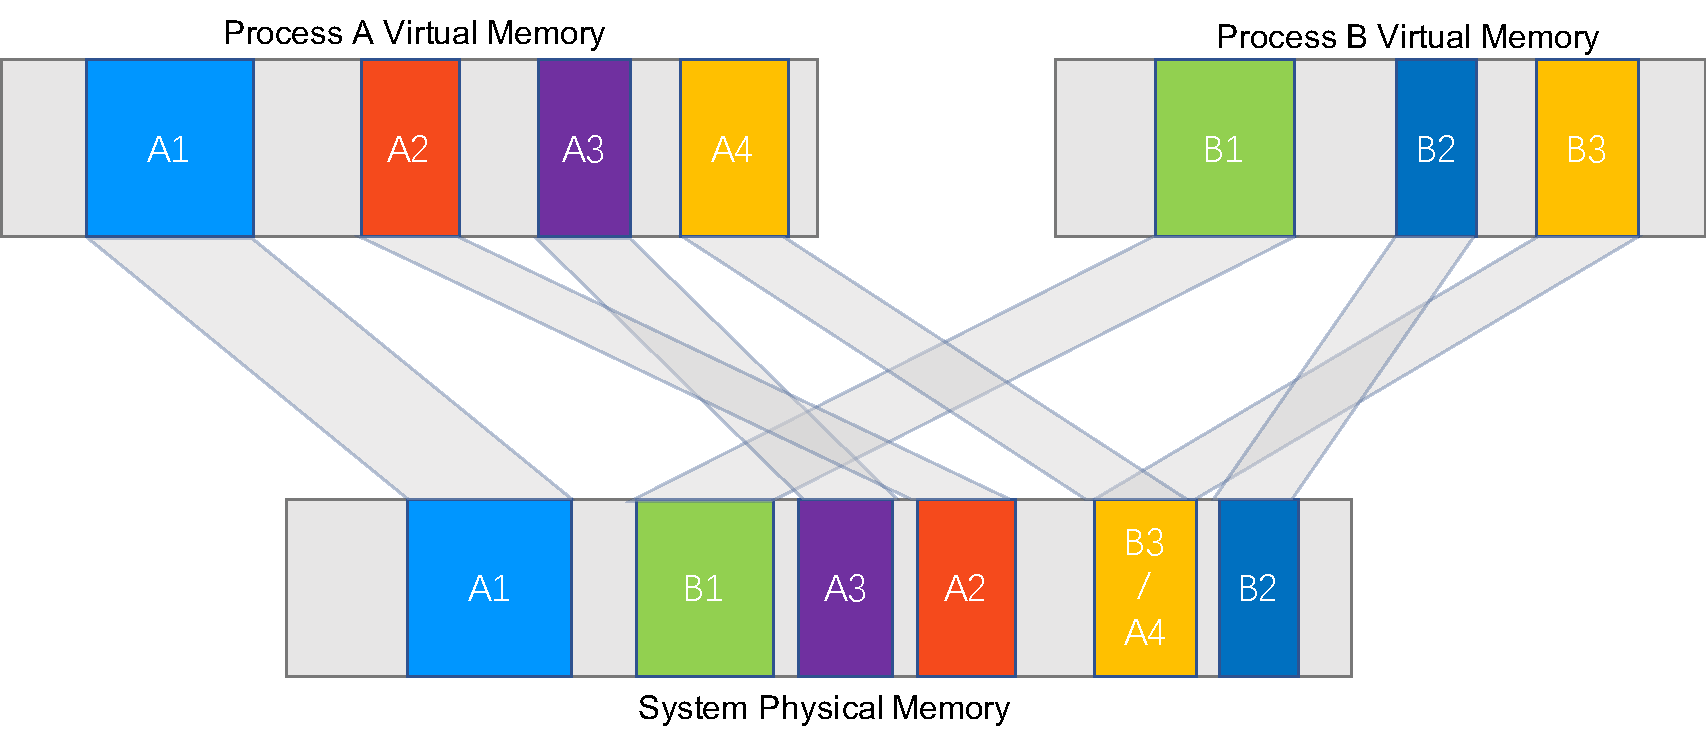
\includegraphics[width=12cm]{memory.pdf}
  \bicaption[Linux虚拟内存映射原理]
    {Linux虚拟内存映射原理}
    {Mechanism of Linux Virtual Memory Mapping}
  \label{fig:MEM}
\end{figure}

由此可见,物理内存页的状态分为三种:没有被映射到任何进程的虚拟内存里(未使用的物理内存页),被映射到唯一的线程的虚拟地址空间里(例如线程的用户栈),被多个进程共享(如共享库);而所有的虚拟页也分为三种:未被映射的虚拟内存页,映射到独占的物理内存的虚拟内存页,以及映射到共享内存的虚拟内存页。如图\ref{fig:MEM}所示,进程A、B的虚拟内存由已映射物理内存的页和未映射物理内存的页组成,其中A1、A2、A3物理页由进程A独占,B1、B2物理页由进程B独占,A4和B3物理页被同时映射到进程A和B的虚拟地址空间中。只要A进程和B进程中的一者对A4(B3)虚拟内存区域作出写操作,另外一个线程即可读到该写操作的内容。而在不共享物理页面的虚拟内存区域进行写操作,则不反映到另一个进程的虚拟地址空间里。这个同步过程是由硬件的缓存一致性机制(cache coherent mechanism)所保证的,当这两个进程中的一者写入后,另一者再次对该区域的内存进行访问,则会引起cache miss(缓存不命中),于是可以读取到内存中最新的内容。

\subsection{非一致性内存访问架构}
历史上,为了提高系统的计算能力,一开始是通过加快CPU的运行频率,直到CPU频率的提高遇到了瓶颈,硬件设计者就设计了多核CPU。越来越多的CPU核通过系统中唯一的北桥来读取内存(这种架构被称为一致性内存访问架构,UMA),当CPU核的数量多到一定程度时,各个CPU核之间对北桥的竞争越来越激烈,内存访问的延迟越来越大,使得北桥(具体来说,是北桥上的集成内存控制器,IMC,Intergrated memory controller)成为计算机性能提升的新的瓶颈。于是硬件设计师将所有的CPU分组,每个Socket上的CPU为一组,系统中有多个Socket。每个socket上的CPU是一个NUMA节点,并且给每个CPU小组分配独立的内存,称作本地内存。每组的CPU在同一个Socket上,共用同一个集成内存控制器,竞争北桥的CPU数量就得到了明显下降,CPU访问本地内存(local access)的速度得到了提高。然而,只有在CPU访问本地内存时延时较短,而访问其他NUMA节点的内存(remote access)就需要经过QPI Interconnect通道,增加了访问时延,故得名NUMA。
\label{chap:memm}

Linux内核使用Node(节点)、Zone(区)、Page(页)三级结构描述物理内存\cite{phymem}。对于UMA架构,内核中只存在一个静态Node结构,而对于NUMA架构,内核可以自由增删Node结构,用Node结构体管理一个NUMA节点的本地内存。每个Zone用于不同的功能,而Page是内存与磁盘交换数据的单位。当Linux进程申请物理内存时,内核优先将本地节点的物理内存分配给这个进程,如果仍未满足需求,则向临近的NUMA节点请求内存页,最终满足内存需求。Linux调度器对NUMA架构做了优化,即当调度发生时,优先选择本地节点上的进程调度。如果本地节点的资源使用率超过了一个界限,则触发负载均衡机制,将该进程从本地节点移动到最合适的节点上。Linux的内存映射机制也对NUMA架构进行了优化。Redhat公司的Rik van Riel提出了Automatic NUMA Balancing(NUMA自动平衡)机制\cite{balancing},经过一段时间(Scan delay)扫描进程的地址空间,将进程虚拟地址空间中的一小部分页面\footnote{一般是256MB}取消映射(unmap)。当进程对这些被unmap的页面进行访问时,会触发NUMA page fault(NUMA缺页异常)。Numa Page Fault向操作系统报告发生page fault的页面的位置,从而得出该进程使用的页面在NUMA系统中分布的位置,从而将进程移动到内存访问最多的节点上。

经过硬件工程师和软件工程师的共同努力,单个服务器装备的CPU数量得到了巨大的提升,单个程序也很难将整个机器跑满,从而促进了云的发展,将海量的物理资源通过虚拟机、容器等形式分发给数量众多的用户,开启了云时代。本文中,巨型虚拟机为客户机提供的是一个NUMA架构的系统,而分布式共享内存(DSM)的性能特性和NUMA架构类似,故针对NUMA架构的优化也可以使用在巨型虚拟机上。

\section{巨型虚拟机架构简述}
\subsection{系统虚拟化简介}
在计算机科学中,增添抽象层次是一个很重要的研究方法。在不同的场景下添加不同的抽象层,得到的结果大不相同。如果将抽象层置于CPU上,则会产生进程的概念,为系统中所有的任务\footnote{Linux将线程和进程都称为任务,task\_struct,不做特殊区分}抽象出可以独占的CPU,从而让CPU被分时复用,从而使得其性能得到最大化的利用。如果将该抽象层置于物理内存之上,则产生虚拟内存的概念,使得进程获得了一个连续的广阔的虚拟地址空间。如果抽象出一个ISA(Instruction set architecture,指令集架构),即一个计算机运行的硬件环境,则是虚拟化(system virtualization)这一重要概念。VMM(虚拟机管理器)可将客户机运行在虚拟的硬件之上,系统虚拟化将操作系统与底层硬件解偶,具有诸多的优势,例如良好的封装性和硬件无关性\cite{sysv},这使得虚拟机可以在任何时候停止执行,通过快照在任何时间任何环境恢复先前的执行,方便了虚拟机的迁移与容错,也促进了数据中心的负载均衡。本文正是利用了虚拟化这个抽象层的这一优点。

历史上,纯软件虚拟化技术的出现早于硬件辅助的虚拟化技术。早期的二进制翻译技术(即将每条客户机指令在执行时进行翻译,类似于解释型编程语言),是完全基于软件的虚拟化。由于软件模拟硬件行为的复杂性,纯软件的虚拟机监控器工程量巨大,代码复杂,同时模拟出的虚拟硬件性能相比于真实硬件有明显下降。之后出现了半虚拟化(Para-Virtualization)技术来弥补纯软件虚拟化方式的不足。其想法是为虚拟机管理器定制客户机OS,使得客户机明确地知晓自己处在虚拟化环境中,与虚拟机管理器相互配合,解决了体系结构造成的虚拟化漏洞。最具有代表性的基于半虚拟化的虚拟机监控器就是Xen\cite{artofxen},Xen运行的定制的guest OS调用Xen的接口配合Xen完成虚拟化功能。但是,由于Windows等闭源操作系统的存在,半虚拟化的可应用范围依然受限。现如今,硬件辅助的虚拟化是应用最为广泛的虚拟化方式。Intel推出的VT-x(Virtualization Technology for x86 processors)技术\cite{intelv}和AMD推出的SVM(Secure Virtual Machine Architecture)技术\cite{amdv}在现有的CPU指令集架构上增加了专用于系统虚拟化的指令,例如Intel的VMX指令(有VMPTRLD、VMREAD、VMWTRITE等)\cite{intelSDM}。x86架构的处理器有根与非根两种运行模式,客户机运行在非根模式,当客户机的特权指令执行时,将触发VMexit,于是CPU运行模式自动转换,使得VMM可以通过trap-and-emulate(陷入并模拟)方式模拟客户机的特权指令。硬件辅助的优点是免去了客户机的修改;又由于客户机指令无需翻译,便可以直接运行在真实的硬件CPU上,使得CPU虚拟化的代价也大大减小。

对于内存虚拟化,传统的方式是为每一个客户机进程维护一个shadow page table(SPT,称为影子页表),代替客户机自带的页表,将其覆盖(shadow),每当进程修改GPT,就需要对SPT进行维护。然而当客户机进程数量较大时,影子页表维护和保存的开销将会十分可观。同时,由于客户机修改自己的页表(GPT)时SPT也要进行相应的修改,VMM将GPT所占的内存标记为写保护(write protected),当客户机修改GPT时会引起VMexit,退出到VMM中由VMM完成对SPT的维护。这对于memory intensive(内存密集)型任务是一种灾难,因为会引起大量的VMexit,严重影响其性能。硬件机制EPT(Extended Page Table)使用硬件维护的GPA到HPA的映射,替代了软件实现的SPT。客户机依然使用自己的CR3指针进行地址翻译,将GVA翻译为GPA,而每一个guest OS都有其对应的扩展页表,EPT base pointer(扩展页表基指针)指向扩展页表(EPT),将GPA通过硬件翻译为HPA。于是,客户机修改自身的GPT(guest page table)时无需引起VMexit,从而使得内存虚拟化的性能相比于影子页表的方式有了很大改进。硬件上也有类似于传统页表TLB(translation look aside buffer)的应用于EPT的页表,缓存了EPTE(EPT表项),加快了由GPA到HPA的翻译。使用本文所使用的巨型虚拟机即利用了这一硬件扩展,实现了内存的高效虚拟化。

VMM又可分为Type-\uppercase\expandafter{\romannumeral1}型和Type-\uppercase\expandafter{\romannumeral2}型。Type-\uppercase\expandafter{\romannumeral1}型又称为Hypervisor型,这个类型的虚拟机监控器直接运行在裸金属上,全权负责虚拟机的创建、调度、运行、电源管理等,是一个完备的操作系统,所以需要编写大量驱动以及操作系统功能,工程量较大,但也具有更好的性能。而Type-\uppercase\expandafter{\romannumeral2}型VMM事实上是host OS的一部分(内核模块),仅仅具有虚拟化的功能,而最基本的操作系统功能由host OS负责完成。还有混合型虚拟机监控器,它同样运行在裸金属上,但是将设备驱动、设备模型的控制权交由一个特权虚拟机。Xen属于混合性虚拟机,它将操作系统应当实现的功能交由domain 0这一特权操作系统完成。然而,Type-\uppercase\expandafter{\romannumeral1}型和混合型虚拟机都要求客户机操作系统进行特定的修改,这对闭源操作系统是不现实的,而且这种修改减小了虚拟化的灵活性,使得操作系统不容易部署在这类虚拟机监控器上,故这两类虚拟机监控器没有得到大范围应用。而开源虚拟机监控器QEMU-KVM属于Type-\uppercase\expandafter{\romannumeral2}型,KVM\cite{KVM}是Linux内核中安装的kernel module(Linux内核模块),而QEMU\cite{QEMU}是运行于用户态的宿主机应用程序,主要负责应对客户机的I/O请求,将KVM作为其虚拟化加速器,KVM利用x86处理器的VT-x、EPT等硬件辅助虚拟化功能获得了更优的虚拟机执行效率,而无需修改客户机操作系统,因此得到了广泛的应用。下一节我们讲述如何对QEMU-KVM进行修改来实现巨型虚拟机。

\subsection{巨型虚拟机架构实现}
巨型虚拟机属于分布式虚拟机,即把一个分布式系统作为运行的物理基础,对上层提供统一的操作系统接口。其主要目的是为了资源聚合,即将分布式系统中的多个普通单机聚合起来,形成一个纵向扩展的虚拟机。例如,普通计算机的CPU核心数目一般在50以内,而更多CPU核心数目的机器则会非常昂贵\footnote{36个CPU核心是服务器较为典型的配置。详见 https://www.quora.com/What-are-the-specs-of-a-typical-modern-server}。有了巨型虚拟机,我们可以将多个普通且廉价的物理机聚合起来,启动一个拥有海量资源的虚拟机,例如将5个配备36个CPU的服务器进行资源聚集,我们可以得到一个拥有180个虚拟CPU的客户机,这是单个物理机很难达到的配置,但又为上层操作系统提供了单一机器的虚拟硬件资源,所以同时具有了纵向扩展系统和横向扩展系统的优势。

巨型虚拟机基于QEMU-KVM这一Type-\uppercase\expandafter{\romannumeral2}型虚拟机监控器(修改后的QEMU称作dQEMU,distributed\ QEMU),将QEMU-KVM扩展为分布式虚拟机。其实现主要分为三个部分,这与系统虚拟化常见的三个需要完成的部分相同:实现分布式vCPU、分布式虚拟内存,以及分布式虚拟I/O。支持巨型虚拟机运行的物理基础是多个物理机组成的集群,在集群的每个节点上,都运行着一个巨型虚拟机的dQEMU实例。每个实例都拥有整个集群的资源,属于本机的资源标记为local(本地资源),而集群中其他节点的资源标记为remote(远程资源)。当本地虚拟机实例对远程资源发起请求的时候,路由模块会找到所访问资源的真实位置,将资源请求转发到真正拥有该资源的节点上。而内存资源是一个例外:所有的虚拟机的QEMU实例拥有全部的内存资源,由DSM(distributed shared memory)进行提供。完成分布式虚拟化的三个主要功能模块有:


\noindent\textbf{分布式vCPU}\quad 巨型虚拟机添加了新的QEMU参数,将一部分本地运行的vCPU标记为local vCPU,而其他未标记的vCPU则是remote vCPU。QEMU为所有的vCPU创建APIC。local vCPU线程在完成初始化之后可以继续执行,而remote vCPU线程初始化完成后阻塞(被调度器放置于睡眠队列),直到虚拟机被销毁。当有IPI(inter processor interrupt,处理器间中断)发送给vCPU时,会向目标APIC的APIC ID寄存器、LDR(Logical Destination Register)寄存器、DFR(Destination Format Register)寄存器写入IPI请求。远端vCPU的APIC称为dummy APIC(傀儡APIC)。dQEMU为每个vCPU在其本地QEMU实例上维护一个真实APIC,而在其他的所有QEMU实例上维护一个dummy APIC。在写入请求时,检查该IPI是否发送给远程vCPU,即检查上述三个寄存器的写入是否是对dummy APIC进行写入。如果是发送给本地vCPU,即向真实APIC写入,则按照原有流程处理;否则,该QEMU实例将对IPI请求进行转发,将IPI注入到远程APIC,同时将集群中所有该vCPU的APIC拷贝强制同步,由远程的QEMU实例接收IPI请求并进行处理。如果集群中有四个节点,每个节点分别运行QEMU 0-3,而每个QEMU实例分别有vCPU 0-3。当vCPU 0向vCPU 3发送中断时,先向QEMU 0中vCPU 3的dummy APIC写入上述三个寄存器,同时QEMU 1-3从QEMU 0得到最新的APIC状态。QEMU 3通过APIC识别出vCPU 3是IPI的接收者,故QEMU 3将IPI注入到vCPU 3。

\noindent\textbf{分布式共享内存}\quad 内存虚拟化模块是巨型虚拟机最关键的部件,为所有的QEMU实例提供了和普通内存完全相同的接口,使得所有虚拟机共享完全相同的虚拟地址空间。普通QEMU为虚拟机分配内存的原理是,通过执行一次mmap()函数,在宿主机虚拟地址空间中分配guest OS物理内存。在分布式共享内存开发的初期,为了尽早测试分布式共享内存的代码,巨型虚拟机在单机上进行测试,将所有QEMU实例的虚拟机内存映射到同一块内存,即对相同的文件调用mmap()函数,从而使得所有QEMU实例拥有共享的内存空间。在开发的后期,在KVM中实现了DSM模块,并与QEMU对接,才转向真正分布式的DSM实现,即通过RDMA或TCP协议进行所有QEMU实例之间内存的同步。

如图\ref{fig:DSM}所示,分布式共享内存(DSM)主要通过维护EPT中页表项的状态,即维护虚拟机所拥有物理内存页的状态,修改EPT的映射,将客户机的物理内存映射到集群中的各个节点。DSM的设计基于Ivy\cite{ivy},Ivy实现了MSI protocol,满足了SC(sequential consistency,顺序一致性)。每个客户机物理页的状态分为Modified:本地vCPU对页作出修改,远程vCPU尚未获得该页的修改,Shared:本地vCPU和远程多个vCPU共享该页,Invalid:需要向其他节点获取该页的最新拷贝,否则本地vCPU无权对该页进行读写。所以,在某个dQEMU实例触发Page fault时,需要使用RDMA协议或TCP协议向远程节点请求最新的数据页。由于巨型虚拟机中的分布式共享内存需要至少实现x86-TSO(Total Store Order)\cite{tso}弱的内存模型,故节点间内存同步的次数和较弱的内存一致性模型相比更多。如果巨型虚拟机的两个节点上的进程相互共享过多的内存,势必会增加内存同步的开销。

\label{chap:DSM}
\begin{figure}[!htp]
  \centering
  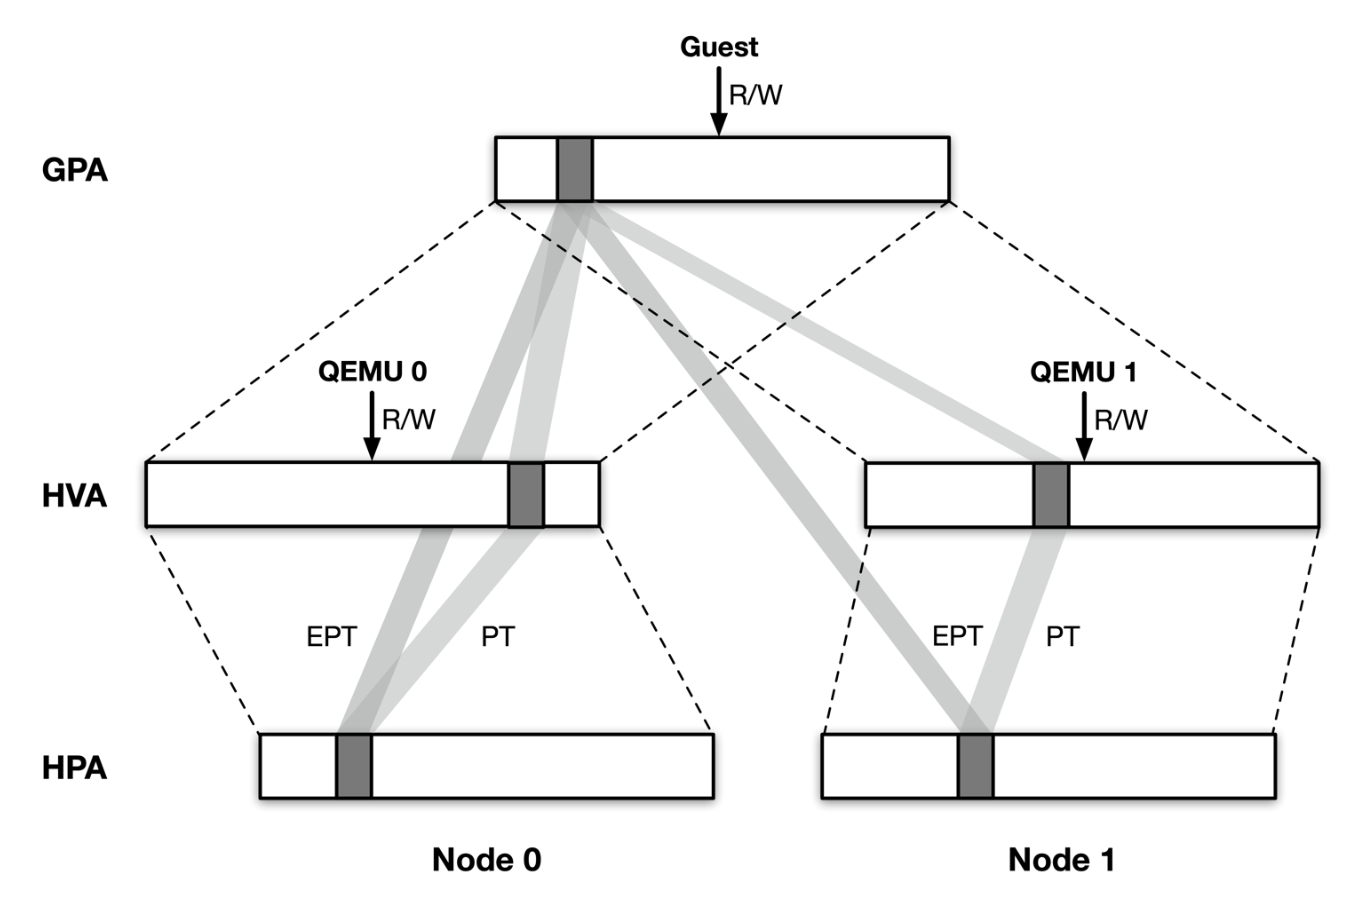
\includegraphics[width=10cm]{dsm.png}
  \bicaption[巨型虚拟机的内存映射]
    {巨型虚拟机的内存映射\cite{giantvm}}
    {Memory Mapping of Giant Virtual Machine}
  \label{fig:DSM}
\end{figure}

\noindent\textbf{I / O虚拟化}\quad 实现分布式虚拟I/O需要解决以下问题:虚拟机vCPU如何对远程节点上的的模拟设备进行I/O访问,以及如何使得远程的虚拟设备产生的中断准确的路由到对应的vCPU。对于第二个问题,分布式vCPU的虚拟化中对于IPI的处理已经给出了答案,即在QEMU 0上放置master IOAPIC,而在QEMU 1-3上放置dummy IOAPIC。在设备中断到达之后写入dummy IOAPIC时,将信息同步至master IOAPIC,由master IOAPIC将中断通过dummy APIC转发给目的vCPU。对于第一个问题,CPU对设备进行I/O访问有两种方式:PIO(Programmed I/O,针对于x86架构)和MMIO(Memory Mapped I/O)。客户机执行I/O指令后退出到VMM,VMM检查I/O指令的目的设备。如果I/O访问的目的设备是远程机器上的设备,则需要将该请求转发给远程设备,在处理完成后将处理结果发送回来。

\section{分布式共享内存性能分析}
\subsection{性能瓶颈}
\label{chap:bottle}
如\ref{chap:DSM}节所述,巨型虚拟机相比于普通虚拟机的实现增加的部分有:(1)分布式共享内存,这一部分需要通过RDMA、TCP等网络协议在集群之间同步物理页的状态;(2)转发机制,将对于远程资源的访问请求转发到对应的节点上去,由真实的资源拥有者处理访问请求。这两部分均会产生网络开销,而网络开销最大的则是分布式共享内存这一组件。顺序一致性是较强的一致性模型,会产生false sharing(伪共享)现象和page thrashing(页面颠簸)现象\cite{sharing}。伪共享现象是指两个运行在不同CPU核心上的线程不断地写入同一个cache line(缓存行)中的变量,当其中一个线程对变量写入后,另一个核上的缓存行即会失效,于是另一个线程需要从内存中读取最新的数据,而写入变量的线程也需要将缓存行写回主存。如此循环往复即出现了伪共享现象。而页面颠簸现象是由于内存页的换入换出。当一个进程频繁访问的页面数量多于总的物理页面数量,或者操作系统为进程选取的驻留集大小(RSS,可以通过ps aux等命令行工具观察进程的驻留集大小)小于其频繁访问的虚拟空间大小,则会有虚拟页面不断换出到磁盘上,即产生了页面抖动现象。

\label{chap:STOR}
伪共享现象和页面抖动现象都是因为不同层次的存储器访问延迟大不相同造成的。现代计算机有如下几个存储器层次\cite{csapp}:
\begin{itemize}
  \item L0 寄存器:在CPU内部用来存储指令和数据。访问时间不超过一个CPU cycle(CPU时钟周期),用于缓存来自高速缓存(L1-L3)的数据
  \item L1-L3 高速缓存(SRAM):静态RAM,L1访问需要几个时钟周期(约为4个时钟周期),L2访问需要几十个时钟周期(约为10个时钟周期),L3访问需要近百个时钟周期(约为40个)\footnote{数据来源:https://v2ex.com/t/523069}。L1分为数据缓存(dcache)和指令缓存(icache),L1、L2由单个CPU核独享,L3由处理器中所有的核共享,保存来自于L4的数据。
  \item L4 主存(DRAM):动态RAM,访问需要几百个时钟周期(100ns),用来缓存来自磁盘的数据。
  \item L5 本地的二级存储,即磁盘(Disk):磁盘分为SSD(固态硬盘)和HDD(机械硬盘),SSD一次读取时间为16,000纳秒,HDD一次读取时间为2,000,000纳秒。
  \item L6 远程二级存储(Web服务器等):经过网络协议与网络进行数据交换,访问时间约为150,000,000纳秒\footnote{数据来源:https://stackoverflow.com/questions/4087280/approximate-cost-to-access-various-caches-and-main-memory}。
\end{itemize}

为了获得更大的内存容量,不可避免的会遭受更高的访存延迟,这对于NUMA架构系统和分布式共享内存是一样的。分布式共享内存增加了物理内存的容量,需要通过网络访问远程节点的内存,相比于本地内存访问增加了网络开销,造成了性能瓶颈。如果在不同节点上的应用程序频繁访问共享的地址空间(如内存密集型任务、I/O密集型任务),则需要分布式共享内存模块进行大量的内存同步工作,不仅造成客户机内存访问的延迟明显提高,使得巨型虚拟机可扩展性降低,还会占用集群中宝贵的网络带宽。虽然分布式共享内存模块已经利用RDMA、压缩优化等技术大大减小了其占用的网络带宽,但仍需要解决根本问题。我们通过设计一个巨型虚拟机客户机的DSM专用调度器,使得节点间访问共享内存的机会更少,增强客户机内存访问的局部性,从客户机的角度解决了根本问题。

\subsection{增强访存局部性的方式}
由\ref{chap:mem}节和\ref{chap:memm}节所述,造成进程之间频繁访问共享内存的原因之一是共享的内核数据和代码。由于对内核数据结构的频繁访问,硬件为了保持缓存一致性,会频繁的从内存中读写数据,造成如上节所属的分布式共享内存所遇到的两个问题。于是,来自ETH Zurich的研究者们从操作系统的内核架构开刀,将宏内核切分开来,实现了一个多内核操作系统Barrelfish\cite{barrelfish}。Barrelfish操作系统将现代的计算机系统视作一个网络,每一个CPU核以及它所附带的缓存是该网络中的一个节点。其设计理念有如下三点:

\begin{figure}[!htp]
  \centering
  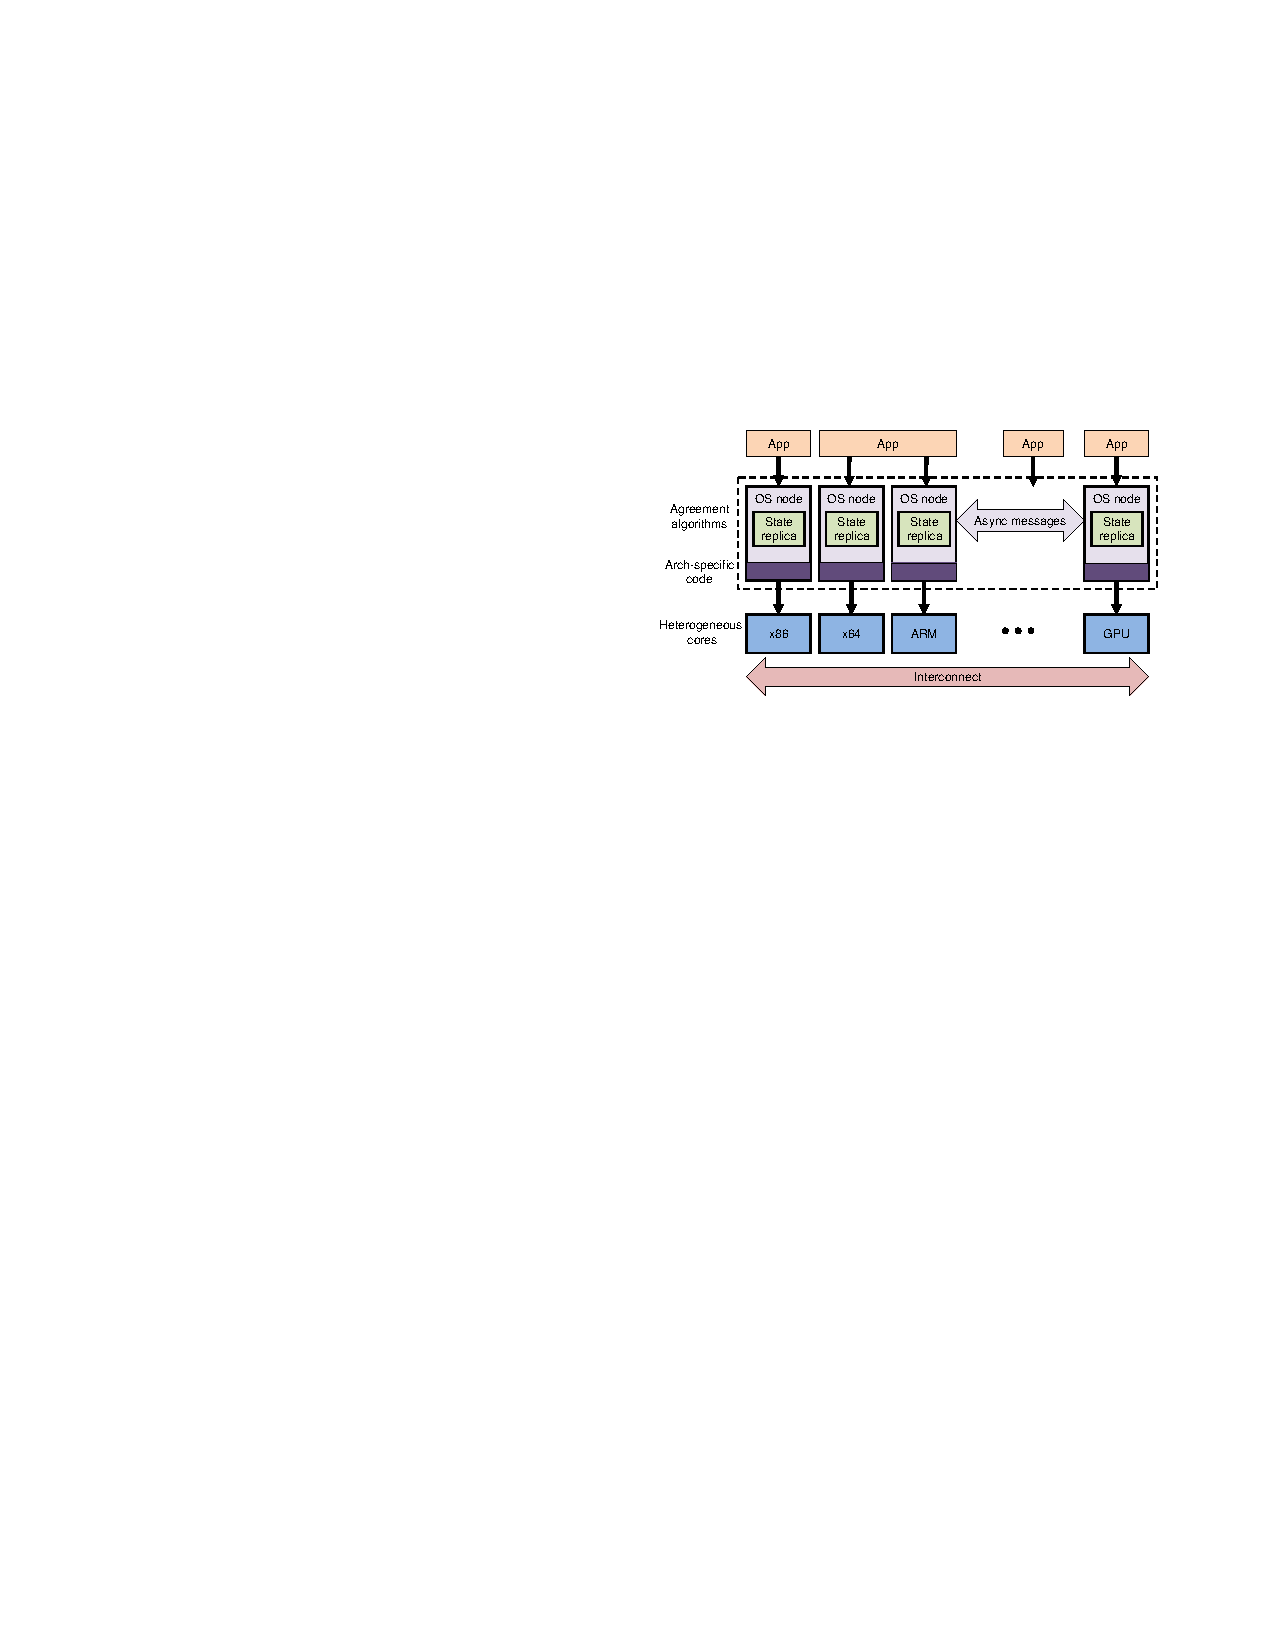
\includegraphics[width=12cm]{barrelfish_sosp09.pdf}
  \bicaption[Barrelfish OS多内核架构]
    {Barrelfish OS多内核架构\cite{barrelfish}}
    {Architecture of Barrelfish OS Multikernel}
  \label{fig:barrelfish}
\end{figure}

\noindent\textbf{核间显式通信}\quad 在宏内核的操作系统中,CPU核之间相互通信大量地依赖于共享内存。然而,如果将单个计算机的硬件视作分布式系统的话,那么将共享内存(shared memory)作为通信的渠道将获得类似于广播的效果:映射了这块物理内存的所有进程都将会通过缓存一致性协议,从内存中获取最新的数据,从而收到这条信息。所以,发送一条信息耗费的时间将会随着硬件系统中的节点数成正比地增加。这是由于CPU在等待缓存一致性机制完成数据同步,从缓存不命中的硬件处理过程中返回,于是发送一条信息的时间也会随着信息量的大小而线性增长。而在消息传递(message passing)模型中,存在服务端线程(server thread)和客户端线程(client thread),服务端线程固定地运行在一个CPU核上,维持着所有客户端线程所需的信息。所有客户端线程只需发送一个远程过程调用(RPC, remote procedure call),虽然远程过程调用所传递的信息依然通过共享内存进行传递,但只是控制面的信息,而真正的数据一直保持在服务端线程的缓存中,不会出现缓存不命中的现象。核之间的相互通信在宏内核中不是显式的,而是通过共享内存隐式地来进行,这样会造成大量不必要的开销。而在Barrelfish操作系统中,核与核之间的通信仅有远程过程调用,而不存在其他类型的通信。故Barrelfish操作系统具有良好的内存访问局部性。

\noindent\textbf{操作系统内核与硬件解耦}\quad 这部分设计理念将操作系统内核的通信算法(策略,policy)与硬件相关的通信机制优化(机制,mechanism)进行解耦合,从而降低工程量。这不在本文的讨论范围内。

\noindent\textbf{全局状态分散为多个副本}\quad 操作系统经常维护一些全局状态,如Linux内核中的runqueue(就绪队列)。当多核时代来临之后,就必须用锁来同步。为了避免锁的开销,常用的办法是将全局状态分解到每一个CPU核上,在Linux 2.4版本\cite{linux}中引入了per-CPU runqueue,极大的提升了调度器的可扩展性,达到了O(1)的运行时间,即调度器运行时间和系统中CPU核的数量无关。在Barrelfish操作系统中,这个概念更进了一步:将所有的内核状态分散在各个CPU核上。如图\ref{fig:barrelfish}所示,内核状态分散在各个CPU核上,只在必要时进行同步。


Barrelfish OS较少的核间通信使得其成为了巨型虚拟机理想的客户机操作系统。即使是如I/O密集型的大量访问内核数据结构的任务运行在Barrelfish客户机中,分布式共享内存也应该具有很好的扩展性。我们分别在Linux和Barrelfish上运行了WebServer,Linux的WebServer是Apache2,而Barrelfish OS的Webserver是调用了Barrelfish操作系统接口的Webserver,所以减少了大量不必要的核间通信。使用ab(ApacheBench)\cite{ab}这一测试工具不断地向WebServer发送GET请求,Barrelfish OS上运行的WebServer比Linux中的WebServer处理速度快6.4倍\cite{giantvm}。这是由于Barrelfish OS将所有的核间通信限制在RPC中,分布式共享内存发生缺页异常的次数也得到了限制,从而减小了网络开销。

\section{数据中心及其资源利用率}
数据中心(Internet Data Center)为内容提供商、企业、政府部门等需要对数据进行保存、共享、操作的组织提供了一个高效安全稳定的运行环境。数据中心由数量巨大的服务器组成(本文将会模拟一个由800台机器组成的数据中心),每个服务器称作该集群中的一个节点,每个节点之间通过高速的网卡进行连接,同时为其提供稳定的电力供应、温控、及时维护等服务,目的是使得数据中心对外提供高质量、稳定的服务。数据中心的搭建还要考虑成本问题,如果将数据中心搭建在气温较低的环境下,则会为数据中心运营者减少很多散热的成本;CPU也为使用者定义了ACPI(Advanced Configuration and Power Interface,高级电源管理接口,其中规范了G-States、S-States、C-States,可以通过调整CPU和整个系统所处的等级来应对不同要求的任务)规范,给软件编写者一个动态调整CPU功耗的方式,从而充分利用CPU,减少功耗成本。而数据中心的资源利用率问题则是数据中心运营者所考虑的关键:如果提高了资源利用率,则意味着可以通过更少的机器对外提供相同质量的服务,同理也意味着可以使用相同的机器提供质量更好、数量更多的服务(例如更高的吞吐量),从而在节约成本的同时,获取更多的效益。提高数据中心资源使用率在一定程度上等同于数据中心的负载均衡:将负载过重的机器上的工作负载迁移到较空闲的机器上,提高了系统总体的并行度,也提高了系统的资源利用率,一些负载均衡的方法也可以达到提高资源使用率的效果。

本文使用基尼系数(Gini Coefficient)\cite{gini}衡量集群CPU资源使用率的均衡情况。基尼系数普遍用于计量经济学,用来表征居民收入的不平均程度。基尼系数是0到1之间的一个数,对于一组完全相同的数据,其基尼系数为0,即最平均;低于0.2则意味着这组数据高度平均,在0.2-0.29之间表示比较平均,0.3-0.39之间表明平均程度一般,0.4-0.59之间则表示同组之间数据差距较大,而在0.6以上则表明这组数据极为不平均。一组全部为1的数据的基尼系数为0,而对于一组均匀分布在0和1之间的数据,其基尼系数为0.333(三分之一),对于有一千个0和一个1的数据,其基尼系数接近于1。我们将其应用在分析数据中心的CPU占用率上,我们认为集群总体的CPU资源占用率的基尼系数在0.25以下表明该集群的负载比较均衡,资源使用率也较高。

历史上,提高数据中心资源利用率的方式有如下三种:

(1)任务混部:这是最符合直觉的一种提高资源利用率的方式,即将更多的任务放在同一个资源较为充裕的机器(或几个机器)中,这样必然使得固定数额的资源得到更好的利用。但是这会对被混部在一起的任务造成影响,由于对资源的更加强烈的竞争,对于某些得不到充足资源的任务,其服务质量将无法达到预期程度,即会遭受QoS\,violation。由于任务的多样性及其工作负载的多变性,资源控制器不能及时地调整任务的混部情况;即使在同一个节点上有很多方式限制一个进程的资源使用量(如cgroup,一种限制单个进程或一组进程的资源使用量的机制),但这依然无法实时地保证每个进程能够获得充足的资源。

(2)工作负载即时采样:通过硬件或者软件的手段对任务的资源占用情况进行即时的采样,根据任务在过去一段时间里的工作负载情况预测未来一段时间内的工作负载情况。例如,最常用的Linux内核所实现的完全公平调度器(CFS,Completely Fair Scheduler)即是采用了这一种策略:在内核表示任务的结构体struct task\_struct中内嵌(由于struct sched\_entity内嵌在struct task\_struct中)一个vruntime变量,记录其已经运行的时间,在每一个调度周期中更新这个变量。每个CPU上的就绪队列维护了一个红黑树,每当一个进程变成可运行状态(RUNNABLE)时将进程按照vruntime添加进入红黑树中,而Linux内核通过vruntime判断在未来一段时间内该进程的运行时间。然而,这样的预测不一定完全准确,甚至有的时候出现完全的预测错误。同时,取样的数据也不一定具有代表性。

\label{chap:reallocation}
(3)资源重分配:为了解决集群中工作负载分布不均的问题,一种更加灵活的方式是将任务在不同的节点上迁移,将资源在任务之间重新分配。迁移的具体方式有进程级别的迁移(Process Migration)、容器的在线迁移(Container Live Migration),和虚拟机的在线迁移(VM Live Migration)。迁移是一种发生在集群节点之间的任务调度,用于平衡集群中节点的负载,进而提高集群的资源使用率。在下面的三节中,我们将对这三类迁移机制进行详细的描述,并且讨论其优劣。

\subsection{进程迁移}
进程级别的迁移主要具有两方面的作用,性能提升和容错\cite{processmigration}。首先是可以得到性能上的提升,进程从较为繁忙的处理器上重新分布到较为空闲的处理器上,使得处理器的负载尽可能均衡,从而提高了系统中进程的并行度和处理器的平均使用率。同时,进程访问物理上较远处的资源会造成更大的通讯开销,例如在非一致性内存访问系统中,访问远程NUMA节点的内存比访问本地内存的开销要大得多,所以Linux内核为适应NUMA架构则将进程迁移到其所访问的内存所在的节点上。其次,进程迁移有助于提高大型系统中的错误包容(Fault Tolerance, FT)能力。现如今,大规模分布式任务可同时使用的处理器已经有成千上万个,在如此庞大的系统中,出现CPU核、内存、网卡、磁盘等部件崩溃的情况越来越多。数据的可靠性可以通过增加副本的方式解决,但会占用额外的资源。进程级迁移为容错提供了一个新的选项,即可以通过一种对软件透明的方式,把遇到硬件崩溃的进程停止,为其进行快照,保存其运行状态,迁移到硬件可以正常工作的环境下恢复进程的执行。进程调度由进程管理线程或由进程自身发起。当该管理线程探测到某些进程满足了迁移的条件,如主机的负载过高,则会向操作系统内核发起一个进程迁移请求,于是被迁移的进程被标记为In Migration,并将其移出runqueue,但其运行状态不被改变。当源主机做好迁移准备后,即向目标主机内核发送一个信息,请求线程的移入,请求附带的信息有进程的资源占用情况和运行状态等。如果目标主机可以接收该进程,则为该进程分配资源。完成分配后,即将源主机上的进程状态复制到目标主机上,同时复制其他进程资源。拷贝完成后,源主机将所有发向该进程的信息转发给目标主机,并等待目标主机上的进程重新恢复执行。最后的任务包括释放源主机上的进程资源,以及恢复目标主机上进程的执行。为了提高进程迁移的效率,有不同的算法被先后提出\cite{migrationppt}。如Lazy copy(延迟拷贝)算法,将被迁移进程从源主机的运行队列里移除之后,首先传输进程在目标主机上执行所需的最小信息,使得进程的In Migration时间缩到最短。但是由于未迁移的状态仍保留在源主机上,如果源主机在进程迁移的过程中崩溃,则被迁移的进程所拥有的信息会遭到丢失,增加了进程的不可靠性。同时,打开的文件、共享内存和发送的信息等资源作为进程间通讯的手段,改变了进程通信的原有语义,会给被迁移进程带来残余依赖性问题。故进程迁移没有被工业界大规模使用,应用程序也很少有对进程迁移的适配。

\subsection{容器热迁移}
\label{chap:containermigration}
容器(container)\cite{container}的出现最初是为了解决应用程序配置部署环境的问题。容器技术将应用程序的运行环境与应用程序本身绑定,将应用程序和其运行环境打包为一个独立的容器镜像,在任何环境下无需重复配置环境即可部署。容器技术同时解决了上述的残余依赖问题,将进程运行在一个具有所有其运行所需的最小资源环境里,与其他进程使用的资源隔离。容器技术因为其轻量、标准化、安全性高等特点,受到微服务(MicroService)架构的青睐。容器相比于虚拟机的启动时间小、内存足迹(memory footprint)小、迁移的网络开销小,可以在同一台服务器上部署成千上万的容器,而虚拟机则拥有整个操作系统的信息,单台机器上无法做到高密度的部署。事实上,一个容器实例是Linux系统中的一个进程,只是和普通的进程相比增加了Namespace、cgroups等运行参数,取消了进程层面上的共享,把残余依赖限制在同一个容器实例中。容器的热迁移\cite{Voyager}具有和进程迁移相似的作用:负载均衡和容错。对于容器迁移的优化目标是缩短Downtime(下线时间),尽可能地减小对服务质量的影响。

内存状态的迁移是容器迁移的主要内容,目前有两种内存的迁移策略:precopy(前拷贝)和postcopy(后拷贝)。对于前拷贝,内存页的拷贝发生在容器迁移之前,即发起迁移请求后,容器继续在源节点上运行,而容器的内存页已经开始向目的节点迁移。在每一轮的内存页拷贝中,不断的有上一轮拷贝至目的节点的内存页被容器修改,所以在本轮中重新传输。在经过一定数量的拷贝次数之后,迁移管理进程发现将拷贝循环继续进行下去将很难把所有内存拷贝到目的节点,此时容器冻结(freeze,停止运行),将所有内存页拷贝至目的节点,并恢复容器的执行。由于这一前拷贝过程中内存页被不断地修改,所以对容器中内存密集型的任务不友好,会产生大量的网络开销。因为容器冻结后被修改的内存页数量比所有的内存页一般更少,所以这一迁移方式的下线时间更短。对于后拷贝,拷贝过程一开始就将容器冻结,并将容器的处理器、寄存器、设备等最小执行状态发送给目的节点,而不发送数据量较大的内存状态,使得容器以最短的下线时间开始执行。然而在目的节点开始执行后,容器进程会产生大量的远程缺页异常(remote page fault),也要等待远程内存页在网络上的传输,导致容器在新节点上开始执行之后的效率十分低下。容器热迁移一般要经历更长的下线时间,对一个运行着MySQL和Elasticsearch的容器进行迁移测试,测得容器内任务的下线时间是2-3秒\cite{Voyager}。

\subsection{虚拟机热迁移}
相比于容器,虚拟机是另外一个虚拟化的层次。容器只是一个操作系统中特殊的进程,只是为容器内的进程提供了虚拟的操作系统接口,而其底层操作系统与宿主机进程共用同一个内核,是操作系统层级的虚拟化。而虚拟机如KVM、QEMU等为运行在其中的进程提供了虚拟的硬件,所以是硬件层级的虚拟化。抽象的层级越低,所涉及的状态占用的内存空间也就越大,但也会有越少的残余依赖。容器将残余依赖限制在容器中,而虚拟机有更好的隔离性,消除了所有进程的残余依赖。虚拟机的热迁移作用于一个客户机操作系统实例(OS instance),容器的热迁移则作用于一个进程,而一个操作系统实例所占用的内存相比于一个操作系统中的进程则要大得多。具体来说,一个运行着MySQL的容器所占用的内存空间仅有256MB\cite{Voyager},而一个Linux客户机所占有的内存高达1GB到几GB。于是,虚拟机热迁移势必会造成更大的网络开销,这是虚拟机迁移优化的重点。

\begin{figure}[!htp]
  \centering
  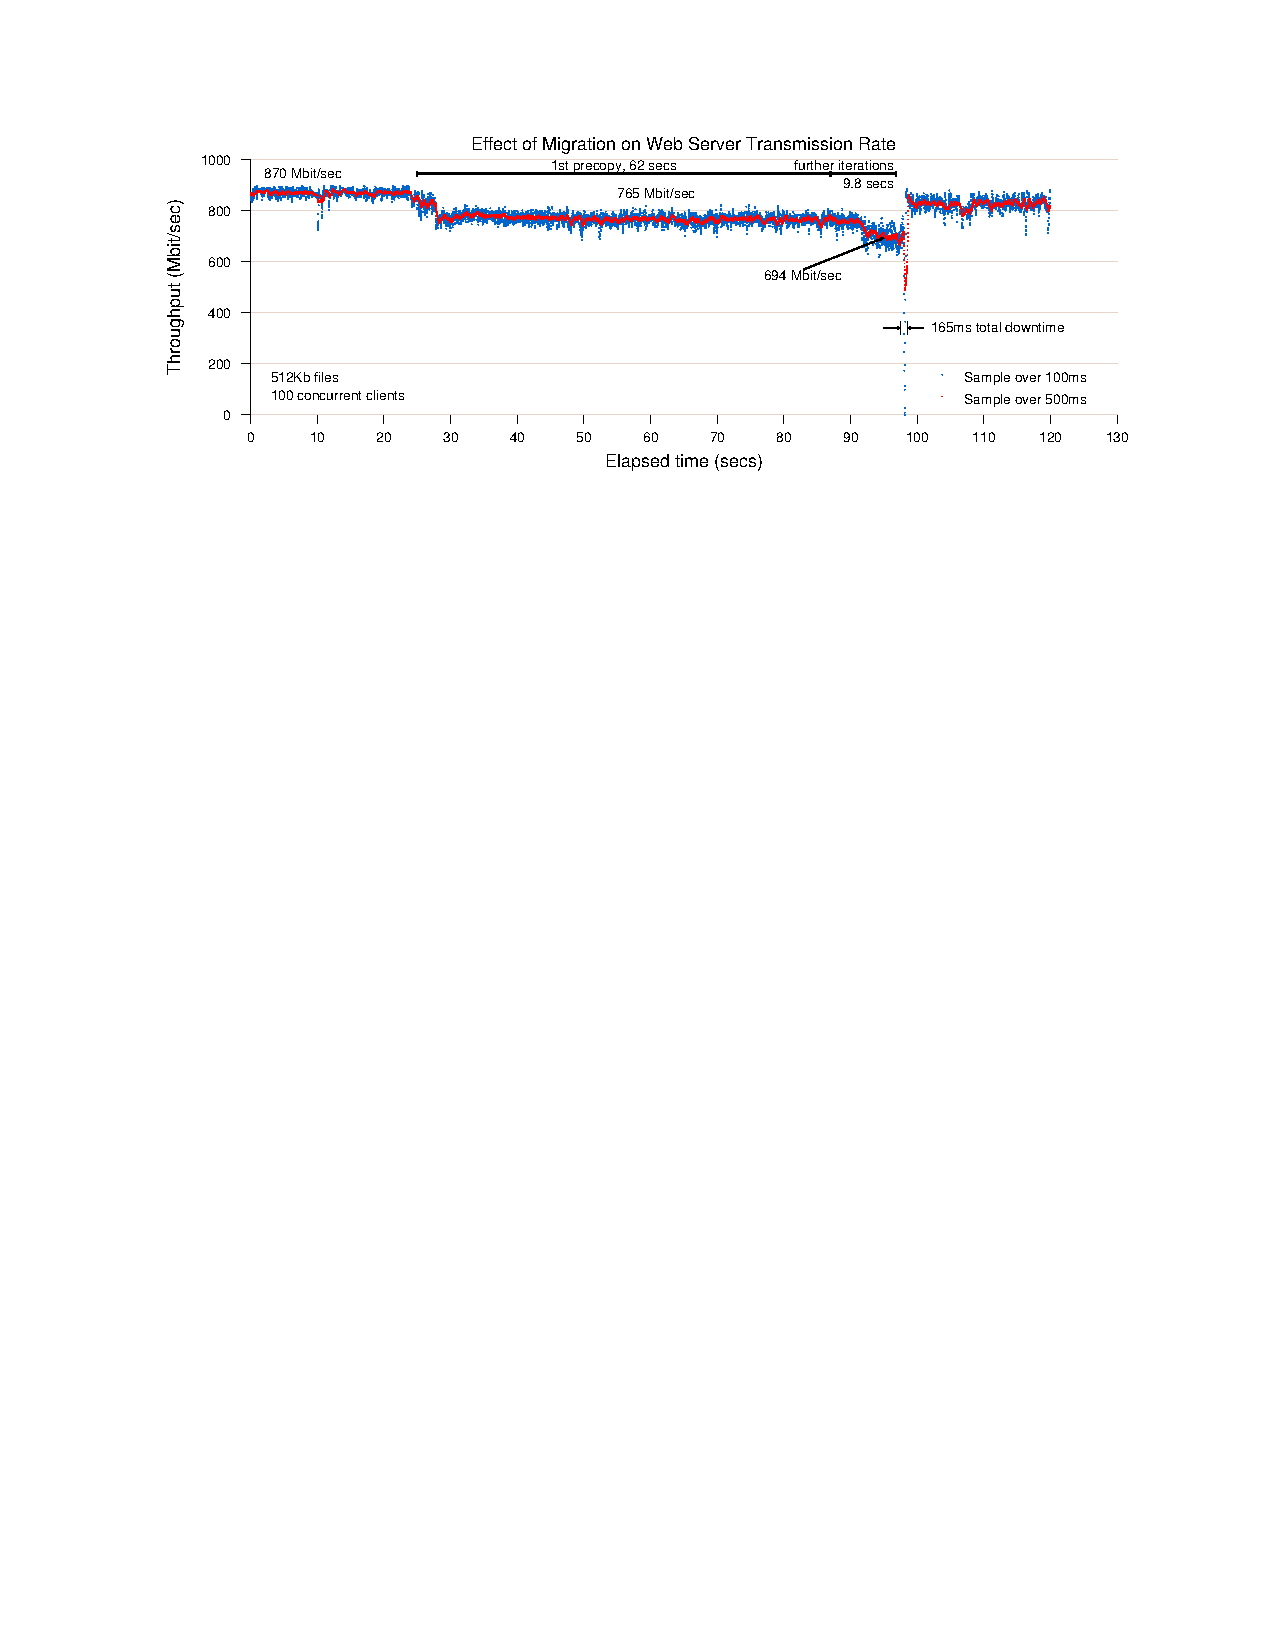
\includegraphics[width=15cm]{vmmigrate.pdf}
  \bicaption[WebServer虚拟机热迁移的网络开销]
    {WebServer虚拟机热迁移的网络开销\cite{livemigration}}
    {Network Overhead of WebServer VM Live Migration}
  \label{fig:livem}
\end{figure}

虚拟机的热迁移\cite{livemigration}分为本地资源的迁移和内存迁移。本地资源在源节点上,虽然像内存和处理器状态等数据可以通过网络发送到目的节点上,而本地的设备例如磁盘、网络接口则无法发送到目的节点,所以对这类资源需要特殊处理。在虚拟机热迁移的过程中,客户机的IP依然保存在TCP PCB(protocol control block,协议控制块)中,不会因为迁移而发生变化,只有其网卡的MAC地址(Media Access Control Address,媒体访问控制地址)发生了变化。源节点和目的节点经常处于同一个由单个交换机连接的局域网中,所以只要让目的节点在此局域网中广播一条包含最新的IP地址的ARP请求(Address Resolution Protocol,地址解析协议,通过IP地址获知网卡的物理地址),当所有的机器接收到这条ARP消息后,即可得知客户机的新MAC地址,这样即可越过源节点,将所有的网络包发送给目的节点上的客户机。而对于本地的硬盘资源,虚拟机热迁移一般依赖于设备整合(Device Consolidation)这一解决方案,如NAS(Network-attached storage)网络存储,由于NAS的地址不会因为虚拟机热迁移而发生变化,所以免去了磁盘迁移的需求。

虚拟机内存的迁移和容器的内存迁移类似,也有前拷贝、后拷贝两种选项,为了使得下线时间尽可能短,且重新启动后较少发生远程缺页异常,一般采用前拷贝的工作方式。虚拟机内存迁移主要分为如下几个步骤:在开始虚拟机的热迁移之前,首先选择资源可以满足迁移来的客户机的节点作为迁移的目标节点,且要求该节点在物理位置上更为临近于源节点,从而不需要远距离的网络传输,出错的可能性更小;接下来就是在虚拟机继续运行的同时对内存页进行循环拷贝,第一轮循环将客户机所有的物理页发送给目的节点,接下来的每个循环依次重传上一个循环中被客户机修改的页。当第$i$个循环重传的页多于第$i-1$个循环时,即表明继续进行内存页传输将是无意义的,于是将虚拟机冻结,再传递CPU、设备等状态,然后传递剩余的内存页,最后在目的节点上恢复虚拟机的执行。虚拟机在目标节点上开始执行后,不会产生远程缺页异常,且下线时间较短。研究人员对一个运行WebServer的VM进行热迁移测试,虽然WebServer服务只有165ms的下线时间,远小于容器热迁移的2-3秒,但迁移过程产生了巨大的网络开销。如图\ref{fig:livem}所示,在这个迁移过程中,网络开销从一开始的870Mbit/sec减小到最后的694Mbit/sec,如此大的网络开销持续了近100秒\cite{livemigration},这对于数据中心的网络带宽是一种极大的占用。

综上所述,不同的迁移方式各有优劣,应用于不同的场景。容器热迁移具有较低的网络开销,但是下线时间较长;而虚拟机热迁移的下线时间极短,但由于其前拷贝的工作方式且虚拟机内存占用较高,所以具有较大的网络开销。数据中心在作出虚拟机迁移决定时一般较为慎重,只在满足了苛刻的条件之后才会进行虚拟机的热迁移。

\section{本章小结}
本章介绍了进程的内存管理方式,以及NUMA架构及其内存自动平衡机制,为后文的理解奠定了知识基础;讲述了本文工作所使用的巨型虚拟机的实现架构,特别是对性能影响较大的分布式共享内存的机制;分析了共享内存的性能瓶颈,并介绍了多内核架构操作系统对分布式共享内存良好的适应性,为高效地使用巨型虚拟机提供了指引;介绍了数据中心的概念和数据中心资源利用率的问题,并提出了三类解决该问题的方法,并详述了各个层面的迁移机制的优劣,进而影响到后文调度器的设计。
%# -*- coding: utf-8-unix -*-
%%==================================================
%% chapter03.tex for SJTU Bachelor Thesis
%%==================================================

%\bibliographystyle{sjtu2}%[此处用于每章都生产参考文献]
\chapter{粗粒度的的调度器设计}
\label{chap:LB}
本章讲述如何利用巨型虚拟机设计一个高效的集群调度器:在不影响集群中任务服务质量的同时,也要提高集群总体CPU资源的使用率。为此,我们提出三条设计理念(设计目标),然后详述我们的设计细节,并且就每条设计目标讨论我们的设计是否达成目标。
\section{设计理念与设计目标}
本文设计调度器应当均衡地将工作负载分配到各个节点上,从而使集群资源得到最大化的利用,这是所有分布式集群调度器都应当达到的目标。此外,我们设计的调度器应当符合如下三条理念:

\noindent\textbf{调度过程开销较小}\quad 一个高效的集群调度器应当尽量缩短任务负载的迁移时间,同时不影响任务负载对外提供服务的质量,否则调度产生的性能提升将被额外的开销与性能影响所掩盖。如第二章第四节所述,集群中的调度可以通过三种迁移方式得以实现:进程迁移,容器热迁移,虚拟机热迁移。进程迁移关注的抽象层次较高,涉及到了操作系统中具体数据结构的迁移,例如和其他进程共享的文件、内存等,目前还没有迁移这些数据结构的方法,所以存在残余依赖的问题。容器的热迁移虽然将残余依赖打包在一个容器实例中,但是有较长的下线时间,对容器内的任务有较大影响,故我们不用容器热迁移作为调度器的实现机制。虚拟机为上层软件提供了简易的硬件接口,抽象层次较低,且带来的下线时间极短,所以我们把虚拟机的热迁移作为关注的重点。虚拟机热迁移的主要问题是,需要迁移整个客户机操作系统的内存,这会占用较大的网络带宽。虽然历史上有一些方法减小虚拟机热迁移带来的网络开销,如并行传送\cite{parallelm}、差分压缩\cite{compression}等方法,但这些方法治标不治本:应当有选择地传输工作负载的状态而非传输整个操作系统的状态,设计一个减小热迁移中传输内存范围的机制,同时尽可能地减小或消除下线时间。

\noindent\textbf{无需修改现有软件}\quad 数据中心内运行的任务种类多种多样,数目巨大,如果调度器需要现有软件的配合才能实现高效的迁移功能,则这类调度器必然无法得到广泛的应用。所以,应当设计一个与现有操作系统(如Linux)适配的且不影响现有应用程序逻辑的调度方法,利用现有操作系统的接口和机制,以减小工作量。

\noindent\textbf{动态感知工作负载}\quad 能够动态地根据节点的工作负载作出最合理的迁移决定是本文的重中之重。相比于设计一个作出单次调度决策的调度器,动态感知工作负载的变化情况,从而作出更多调度决策,必然能够更加充分地使用资源。有两类方式根据工作负载作出迁移决定:主动式决策(proactive)和被动式决策(reactive)。主动式决策通过对系统的精确采样,主动预测工作负载的变化情况(例如使用机器学习技术建立模型,使用以往的工作负载数据训练该模型),作出调度决策。在这类方式中,为了使采集的数据具有很好的代表性,要进行更加频繁的采样,会造成巨大的开销;其次,工作负载的变化情况本身并不可预知,虽然一些运行时间较短的任务有着较为固定的工作负载变化模式,但这些任务对集群整体产生的影响十分有限。故我们选择被动式的决策方式,在系统负载发生改变之后,以最快的速度根据负载情况的变化完成任务调度,即可适应不断变化的工作负载。

\section{粗粒度调度器的设计}
我们受到Barrelfish操作系统设计理念的启发:Barrelfish将操作系统内核状态分割成多个副本,每个副本固定在一个独占的CPU核上,从而避免了基于缓存一致性这一硬件机制的大量核间数据的传输,提高了操作系统的可扩展性。我们将此概念进一步延伸,从而达到我们的目的:虚拟机热迁移所带来的网络开销中含有不必要的操作系统内存的部分,可以将客户机的大部分状态固定在不同的节点上,从而在迁移客户机内部工作负载时,无需传输和工作负载无关的状态,其中包括客户机操作系统的大量数据和代码,以及客户机中其他任务的状态,只传输工作负载所拥有的状态即可(如其频繁访问的内存页)。为达成这个目的,我们需要一个运行在一个分布式集群上的分布式的虚拟机。这样一来,客户机的大部分内存页均匀地分布在集群的每个节点上,就免去了大量内存页的迁移需求。巨型虚拟机基于现有的单机虚拟机管理器QEMU-KVM,开发年限较长,与现有系统的兼容性良好,且运行稳定,可以运行主流的操作系统,所以我们选择巨型虚拟机实现上述目标。

\subsection{迁移机制概述}
\begin{figure}[!htp]
  \centering
  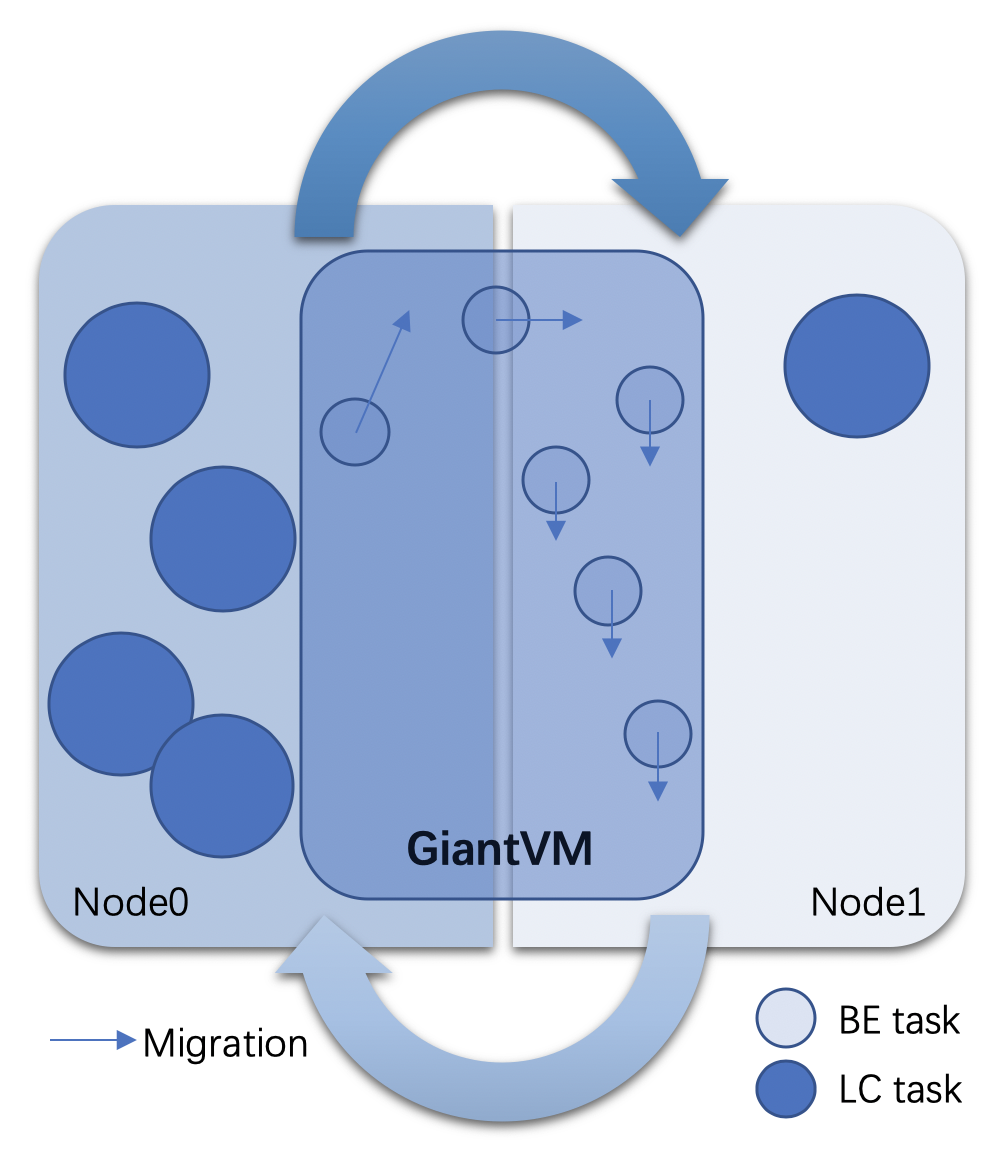
\includegraphics[width=8cm]{schedule.png}
  \bicaption[基于GiantVM的任务迁移机制]
    {基于GiantVM的任务迁移机制}
    {Task Migration Mechanism Based on GiantVM}
  \label{fig:schedule}
\end{figure}

我们将巨型虚拟机$GiantVM$作为集群节点之间交换任务负载的桥梁:将任务分为可迁移任务(migratable tasks)和不可迁移任务(fixed tasks),巨型虚拟机在集群中传输可迁移任务来进行负载均衡。在图\ref{fig:schedule}中,颜色较深的圆圈代表不可迁移任务,系统通常为其分配较充足的资源,故用大圆表示,而颜色较浅的小圆代表可迁移任务,系统无需为其保证充足的资源。巨型虚拟机横跨多个节点来运输可迁移任务。在每个迁移周期中,我们扫描整个系统内的所有进程,选择一部分可迁移进程加入巨型虚拟机的客户机中。巨型虚拟机对客户机提供一个虚拟的NUMA硬件环境,每一个NUMA节点代表分布式集群中的一个节点,从而使得客户机得知底层硬件环境的拓扑结构。我们在客户机中设计一个专用的调度器,它可以动态感知每个NUMA节点下的真实物理节点的负载。当迁移条件满足时(如宿主集群某个节点CPU占用率超过阈值),调度器读取每个节点的负载,选取负载最低的节点,将可迁移任务调度到该NUMA节点上。被迁移的任务虽然不会有下线时间,但是由于分布式共享内存组件的存在,需要对一部分内存页进行迁移,也会在迁移后发生一些page fault,造成一定的性能影响。借助于巨型虚拟机,任务在集群中的迁移过程被简化:客户机中的进程向运行在其他NUMA节点的vCPU上迁移即等同于进程在集群节点间迁移。如图\ref{fig:schedule}所示,Node0中不可迁移型任务对系统资源占用过高,于是触发了可迁移任务向负载更低的Node1进行调度,然而这个调度过程仅发生在巨型虚拟机的客户机内,由客户机内的调度器完成。

至于如何将任务分类为可迁移任务和不可迁移任务,目前的实现是把延迟敏感型任务(LC tasks)作为不可迁移任务,它们不能承受性能的损失(例如一些业务进程,如果延迟提高则会使得收益受到影响),而将尽力而为型任务(BE tasks)作为可迁移任务,其延迟增长对用户的影响不大(例如一些用于开发实验的进程,为了测试未投入使用的代码,或一些数据分析程序)。在图\ref{fig:schedule}中,LC型任务即不可迁移任务,BE型任务即可迁移任务。在这样的分类之下,延迟敏感型任务的服务质量将不会受到影响,而尽力而为型任务将延迟敏感型任务未使用的资源利用起来:由于延迟敏感型任务无法承受性能损失,系统为其分配了足够多的CPU资源,来应对其可能出现的CPU利用率突增,然而大部分时间内这些CPU资源大部分都无法完全利用,于是当延迟敏感型任务占用较低时,巨型虚拟机将尽力而为型任务调度到对应的节点上,填补CPU使用率的空缺,从而提高了集群总体的CPU资源占用率;在延迟敏感型任务占用较高时,巨型虚拟机及时将尽力而为型任务迁移到占用较低的节点上,不与延迟敏感型任务抢占资源,从而保证延迟敏感型任务的服务质量。

\subsection{调度脚本实现}
\begin{figure}[!htp]
  \centering
  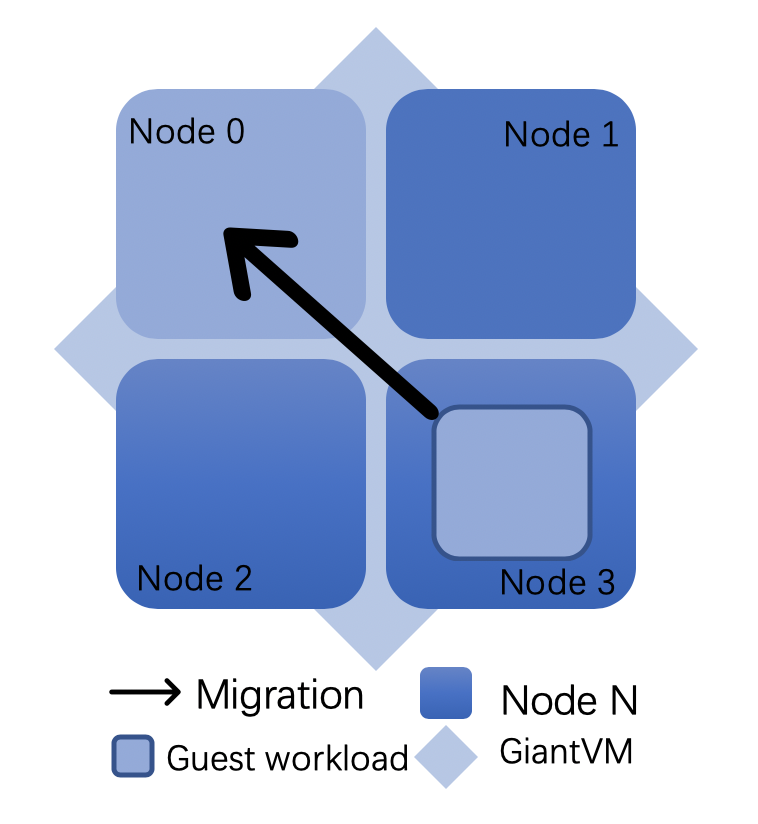
\includegraphics[width=6cm]{coarse.png}
  \bicaption[基于巨型虚拟机的粗粒度的调度]
    {基于巨型虚拟机的粗粒度的调度过程}
    {Coarse Grained Scheduling Based on GiantVM}}
  \label{fig:coarse}
\end{figure}

\begin{algorithm}[h]
\begin{algorithmic}[ruled,1]
\Function {set\_affinity\_all}{$node$}
\If{$current\_node &= &= node$}
\State $return$
\EndIf
\State $node\_cpu\_list \gets get\_node\_cpu\_list(node)$
\For{each $task, irq, wq\in OS$}
\State
\Call{set\_affinity}{$task, node\_cpu\_list$}
\State
\Call{set\_affinity}{$irq, node\_cpu\_list$}
\State
\Call{set\_affinity}{$wq, node\_cpu\_list$}
\EndFor
\State $current\_node \gets node$
\EndFunction
\State
\State $/*\ At\ system\ start,\ pin\ all\ tasks\ to\ node0\ to\ boot\ faster\ */$
\State
\Call {set\_affinity\_all}{$node0$}
\State
\While{true}
\State
\Call {sleep}{$INTERVAL$}
\If {$current\_node.stealtime < 50$}
\State $continue$
\EndIf
\State $/* Migration\ is\ triggered */$
\State $min\_stealtime\_node \gets find\_min\_stealtime\_node()$
\State
\Call {set\_affinity\_all} {$min\_stealtime\_node$}
\EndWhile
\end{algorithmic}
\caption{粗粒度进程调度算法}
\label{algo:coarse}
\end{algorithm}
事实上,上节所述的调度机制应当使用C代码来实现,即在Linux内核中添加一个新的调度器类\footnote{Linux内核中有多种调度算法,每种调度算法自成一个调度器类,由核心调度器调用。现有的调度类有完全公平调度类、实时调度类、空闲调度类}。然而操作系统已经给用户层提供了足够多的接口来实现我们所说的调度策略,而增添一个新的调度器类工作量较大,调试各类参数比较困难,故我们选择使用shell语言实现调度算法。目前在Linux上使用shell脚本实现了一个粗粒度的调度算法,而细粒度调度算法的shell实现作为未来的工作。

对于粗粒度的调度算法,如图\ref{fig:coarse},我们通常将巨型虚拟机部署在四个节点上,只需要找到四个NUMA节点中宿主机占用最低的节点,将客户机中所有的任务迁移到该NUMA节点上即可(颜色深的节点代表其负载较高)。客户机中调度脚本的实现如算法\ref{algo:coarse}所示,我们设置该脚本作为系统启动项。系统启动时,首先调用$set\_affinity\_all()$使得OS中所有的活动都运行在Node0上,Node之间无需做网络通信,缩短了启动时间。此后,每个调度周期中,读取两次累计的steal time做差得到该时段内的steal time,如果当前所有进程运行的节点的steal time超过了一个阈值(50个节拍),即触发迁移,调用$set\_affinity\_all()$将所有OS活动固定在steal time最低的节点上。虽然这样减少了客户机中进程可以使用的虚拟CPU个数,但是最大程度的减少了网络的开销:由于任何两个NUMA节点之间无需共享内存数据,只有一个NUMA节点上有任务在运行。

$/proc$文件夹是Linux内核为用户态程序提供内核信息的文件夹,用户态程序也可通过写入$/proc$文件夹中的某个文件更改内核的配置。在本文中,我们读取$/proc/stat$文件的内容完成两个功能:一是获取宿主机节点上的CPU使用率,二是在客户机操作系统中获取$steal time$。$/proc/stat$文件包含了自系统启动以来累计的CPU节拍数,CPU空闲的节拍数,以及因为虚拟化所产生的累计的$steal time$。$steal time$指虚拟CPU等待物理CPU执行其他宿主机指令或者其他虚拟CPU的时间,直接向客户机反映了宿主机的工作负载状态。在得知了$steal time$最低的节点之后,我们应当尽可能地让所有的Guest OS活动都运行在$steal time$最低的节点上。在Linux中,可以设定CPU affinity(CPU亲和性)的OS活动有\footnote{见内核文档https://www.kernel.org/doc/Documentation/kernel-per-CPU-kthreads.txt的介绍}:

(1)$task\_struct$(进程):可以通过$taskset$命令或者$sched\_setaffinity()$系统调用使得所有的进程线程都运行在指定的CPU列表上,其实现是通过修改$task\_struct$中的$cpu\_mask$这个位图来限制进程线程运行的CPU列表。这类方法无法设定一些内核线程的CPU亲和性,例如$ksoftirqd$, $kworker$等线程;

(2)$irq$(中断处理函数):中断处理函数不对应于任何一个$task\_struct$,故$taskset$无法设定其CPU亲和性。可以在停止$irqbalance$服务(该服务会在所有CPU核上对中断处理进行负载均衡)后,写入/proc/irq/[0-9]+/smp\_affinity文件来限制中断处理函数可以运行的CPU列表;

(3)$workqueue$(工作队列):有一些$workqueue$在$alloc\_workqueue()$时使用了参数$WQ\_SYSFS$,使得我们可以通过$sysfs$文件系统获知并控制其状态。我们写入$/sys/devices/virtual/workqueue/*/cpumask$来设置$workqueue$的CPU亲和性;

(4)$local\ timer\ interrupts$(本地时钟中断):当时钟中断发生时,客户机的vCPU访问了很多时钟中断处理函数相关的内存页,导致这部分内存页在节点之间来回传输。时钟中断在x86架构上较为频繁,一般在一秒钟内有100到1000次的本地时钟中断。虽然tickless kernel通过不向空闲的CPU发送时钟中断(tickless CPU)缓解了时钟中断频繁的问题,但是系统中必须有一个非tickless的CPU,负责完成系统的计时工作。假如Node0上的vCPU0是整个系统中的非tickless vCPU,当我们的调度器将客户机内所有工作负载调度到Node1上时,Node0和Node1之间就会出现频繁的时钟中断相关内存页的交换,产生较大的网络开销,影响任务的性能。根据内核文档的描述,设置内核编译选项CONFIG\_HOTPLUG\_CPU=y后,将空闲Node上的vCPU全部下线($offline$),系统将不会向下线的vCPU发送中断,从而避免了时钟中断的开销。但是我们无法得知下线vCPU的$steal time$,只能随机选择一个node作为调度的目标。事实上,可以通过半虚拟化的方式向客户机通知宿主机上的工作负载,但本文目前未采用这一方案。

\subsection{性能优势}
巨型虚拟机的进程调度等价于虚拟机热迁移,且迁移开销较低,没有下线时间,比较适合资源重分配的集群负载平衡方式(见第\ref{chap:reallocation}节,资源重分配同步于系统中频繁变化的负载,迁移的频率较高)。当巨型虚拟机中的进程被taskset到某一节点上时,由于分布式共享内存模块的内存同步协议,会产生大量的EPT缺页异常,会使得被迁移任务的服务质量严重下降。发生EPT缺页异常后,分布式共享内存模块开始传输该进程的页,直到该进程频繁访问的页被完全传输到目标节点。虽然巨型虚拟机的进程调度会造成缺页异常,引起性能下降,但是其开销还是远小于虚拟机热迁移的开销,因为分布式共享内存只会在各个节点之间传输被频繁修改的页,而非整个客户机的所有内存页。根据第\ref{chap:mem}节对于进程虚拟内存空间分布的分析,我们以客户机的物理页为中心讨论巨型虚拟机相比于虚拟机热迁移无需传输哪些页(EPT将客户机物理页映射到宿主机物理页,故讨论客户机物理页即是讨论宿主机物理):(1)所有被客户机内进程映射为只读的客户机物理页,包括内核态和用户态的.text 段和.rodata段。(2)未被映射进入任何客户机进程的虚拟地址空间以及内核虚拟地址空间的物理页。(3)Linux进程有一个当前进程频繁访问的物理页面的集合。由于数据访问的局部性(data/space locality),进程通常有一个固定大小频繁访问的内存区域,故客户机有部分物理内存虽然被映射进入某个虚拟地址空间,但进程很少访问它们。以上三类页面是虚拟机热迁移机制无法区分的,在迁移一个完整的虚拟机时,必须将其所有使用的宿主机物理页面全部进行迁移。

综上,相比于虚拟机热迁移,巨型虚拟机的进程调度开销较小,满足了第一条设计理念;只需在客户机中添加一个调度脚本,原有软件可以无需修改地运行在客户机上,满足了第二条设计理念;通过读取$steal time$动态感知工作负载,将所有客户机进程迁移到负载最低的节点上,满足了第三条设计理念。

\section{本章小结}
本章提出了三个集群调度器的设计理念,并且描述了如何使用巨型虚拟机完成集群调度功能,以及其shell脚本实现的粗粒度进程调度算法,动态感知负载情况。本章设计的shell脚本的实现可以在任何Linux操作系统中部署,无需修改现有软件,并且相比于虚拟机热迁移大量缩减了被迁移的页面范围,具有较高的迁移性能,无下线时间,达到了本章开始设定的设计目标。
%# -*- coding: utf-8-unix -*-
%%==================================================
%% chapter04.tex for SJTU Bachelor Thesis
%%==================================================

%\bibliographystyle{sjtu2}%[此处用于每章都生产参考文献]
\chapter{基于集群仿真的调度器设计}
虽然在直觉上,基于巨型虚拟机的调度器可提高集群的CPU使用率,但目前我们无法在大型集群上验证我们的实现,同时在大型集群上验证的耗时过长,不易及时发现调度器的性能瓶颈并且快速调整相关参数。本章利用谷歌提供的大型集群中任务调度与任务资源使用情况的追踪数据(trace data)模拟大型集群中真实的任务负载,对之前提出的调度策略进行仿真,并优化其调度算法。在开始使用追踪数据之前,应当对追踪数据的内容有大致了解。

\section{集群追踪数据简述}
本文使用的集群追踪数据(trace data)来自于谷歌的Borg集群(称为cell),包含了一个含有12.5k台机器的集群在29天的追踪周期里的运行情况。具体来说,我们用于集群仿真的数据是ClusterData-2011-2,从北美东部夏令时2011年五月一日的19点整开始进行追踪,持续了29天。较长的追踪时间和较大的机器数量保证了追踪数据的代表性和说服力,能够真实地反应分布式集群的任务负载及其调度情况。Borg\cite{borg}是谷歌在2015年提出的分布式集群调度框架,对于一个Borg集群(称为cell),有一个对应的Borg Master,而每个节点上运行一个Borglet,与Borg Master通信,作出资源分配决策。Borglet计算任务负载并将计算结果放在缓存中,并与Borg Master沟通需要进行的操作,但不与Borg Master频繁沟通,为了防止Borg Master负载过重而宕机。Borg使用容器做到了资源的细粒度分配与限制,资源用量数据通过容器来测量。追踪数据分为对以下几个方面的数据的记录:机器事件(机器加入或离开集群,以及配置更新)、机器属性(包含对机器内核版本、硬件配置、网络配置等多个属性),以及作业(Job)和任务(Task)事件表,记录了作业和任务的生命周期,以及任务在各个采样时间段的资源用量情况。在任何一组数据中,都含有一个或几个时间戳。追踪数据中的时间戳是一个64位的无符号整数,从追踪时间段的前600秒算起,这是为了支持两个特殊时间戳:0代表发生在追踪时间段之前的事件,而$2^{64}-1$(最大的64位无符号数)表示发生在追踪时间段之后的事件。丰富的数据类型对集群的工作状态进行了详细的描述,利用这些数据可以完整地复现一个真实大小的集群,相比于在真实集群上进行测试,可以相当快速地完成模拟。

本文主要使用追踪数据中的两组数据来模拟不同的调度策略:$task\_usage$,每个采样时刻的任务资源用量数据和$task\_events$,任务调度状态变更事件数据。在每一条$task\_usage$数据是各个采样间隔的任务资源用量数据,需要关注的字段有:(1)采样时间段的起始时间和终止时间,(2)任务号,进程号,用于标识一个唯一的进程。(3)平均CPU使用率,最大CPU使用率,(4)用户可访问的内存页数目、最大用户可访问内存页数目、分配给整个容器进程的内存页数目(包括部分用户不可访问的内核页面)。这些数据都是通过测量容器的内存占用量获得的。(5)performance counter相关数据,CPI是平均每条指令花费的CPU周期数,MPI是平均每条指令访问内存的次数。注意,所有资源用量数据均是对最大值标准化过的,例如,所有进程的CPU使用量是1,2,3,4,则在数据中是1/4,2/4,3/4,4/4。在每一条$task\_events$数据是任务事件(包括$SUBMIT$、$SCHEDULE$、$EVICT$、$FAIL$、$FINISH$等)的列表,需要关注的字段有:(1)任务事件发生的时间戳,记录了该任务事件发生的时间点。(2)任务号,进程号,用于标识一个唯一的进程。(3)任务优先级。在追踪数据中,任务的优先级最高为11,最低为0,优先级高的进程可以抢占优先级低的进程的资源。其中几个特殊的优先级有:空闲优先级(0-1),这是最低的优先级,基本不要求资源;产品优先级(9-11),是集群中最高的优先级,调度器避免这个优先级的进程资源被挤占;监控优先级(12),用于监控其他任务的健康状况。(4)CPU、内存资源请求量:进程使用资源的上限,超过这个限制的进程会被限制或杀死。(5)事件类型:标识了进程生命周期中的事件类型。主要的进程事件有:(1)$SUBMIT$:进入$PENDING$状态,进程有资格被调度运行;(2)$SCHEDULE$:进程被调度运行进入$RUNNING$状态,开始真正的占用系统资源(3)$FINISH$:进程正常退出,由$RUNNING$状态变为$DEAD$状态。

\section{粗粒度调度器的仿真}
做集群模拟之前,需要做一些简化假设:
\begin{itemize}
  \item 假设任何一个被$SUBMIT$的进程都将被调度到任意的节点上,集群中除了巨型虚拟机中的调度器外再无集群调度器;
  \item 集群中的机器数量在运行过程中没有变化,没有机器宕机也没有新机器加入集群,每个机器的处理能力也不随时间变化
  \item 网络开销仅计算进程迁移时进程所拥有的内存页(本文选取分配给整个容器进程的内存页)迁移造成的开销;
  \item 网络数据传输不耗费时间,且网络状态始终保持良好,不会出现network partition(网络分割),没有网络带宽的限制。
  \item 假设巨型虚拟机运行不占用节点上的资源,dQEMU进程和DSM不占用CPU和内存。
\end{itemize}

\subsection{仿真系统的建立}
在上述假设成立的条件下,我们用Python脚本(simulator.py)模块化地设计如下仿真系统:
\begin{figure}
\centering
\begin{minipage}[c]{0.55\textwidth}
\begin{lstlisting}[language=python]
class Scheduler:
    def __init__(self):
        self.machines = []
        self.average = []
        self.gini = []
        self.exceeded_load = []
        self.machines=[Machine(i) 
          for i in range(n_machines)]
        self.migration_mem = 0.0
\end{lstlisting}
\end{minipage}
\begin{minipage}[c]{0.55\textwidth}
\begin{lstlisting}[language=python]
class Task:
    def __init__(self, task_id, duration,
        priority, request, usage):
        self.running_start = 0
        self.schedule = 0
        self.duration = duration
        self.priority = priority
        self.request = request
        self.usage = usage
\end{lstlisting}
\end{minipage}
\begin{minipage}[c]{0.5\textwidth}
\begin{lstlisting}[language=python]
class Machine:
    def __init__(self, machine_id):
        self.machine_id = machine_id
        self.tasks = set()
        self.tasks_completion = []
        self.pending = set()
        self.request = 0.0
\end{lstlisting}
\end{minipage}
\end{figure}

\noindent\textbf{进程类(Task)}\quad \label{chap:task}进程类表示一个可以被集群调度的实体,占用集群资源。进程类中的字段有:每个进程的进程号,优先级,CPU使用率上限,和一些时间戳,包括被调度的时刻$schedule$),开始运行的时刻$running\_start$,以及在资源没有被挤兑或抢占时应该获得的运行时间$duration$,还有每个追踪时间段的资源用量列表(包括平均CPU使用率,最大CPU使用率,以及分配给整个容器进程的)。在读取$task\_events$数据时,将$SUBMIT$事件的时间戳填入到Task类的$schedule$字段中,表示进程被调度到某个机器上(不一定开始运行);将$SCHEDULE$到$FINISH$的时间差填入$duration$字段,表示进程以最充足资源完成所消耗的时间;将CPU使用率上限填入$request$字段。在读取$task\_usage$数据时,将$usage$字段用每个追踪时间段的资源用量列表填满。于是,我们可以通过Task的$duration$字段与等待被调度运行的时间之和($duration + schedule - running\_start$)判断QoS violation的程度(称作$duration$),即服务质量的影响程度。$duration$表征了一个任务从被调度到运行完成所用的时间,若任务不合理分布则$duration$值较大。

\noindent\textbf{机器类(Machine)}\quad \label{chap:machine}机器类表示集群中的一个节点,可以和其他任何节点进行网络通信,具有固定的处理能力和负载能力。机器类中的字段有:机器编号$machine\_id$,被调度到该机器上的的所有进程的集合(分为正在运行)$tasks$、等待被调度运行的进程集合$pending$,以及每台机器的容载能力$cap$和当前的负载$request$。每个机器的容载能力设置为$0.5$。当任务被提交到某个机器上时,如果该机器还可以容纳这个任务的负载,则该任务被加入到$tasks$集合,并且将该进程的负载累加到$request$字段,并将该任务的$running\_start$字段置为当前时间戳;如果机器无法容纳该任务的负载,则将该进程加入到$pending$集合,等待其他任务的完成再开始运行。我们通过Machine类提供的$get\_usage(timestamp)$接口来统计某个时刻机器上所有进程的CPU使用量,即当前机器的负载。我们将本机器的负载与实际容载能力相减($get\_usage(timestamp) - cap$)来判断机器$overcommit$(超量提供)的程度,从而得知任务负载是否合理分布。$overcommit$表征了机器上任务负载超过其容载能力的情况,若任务不合理分布则$overcommit$值较大。

\noindent\textbf{调度器类(Scheduler)}\quad \label{chap:scheduler}这是模拟系统中的核心类,是整个集群的任务调度器。在任务调度器类被创建时,它初始化其所拥有的所有机器类。它包含一个$schedule()$接口,用于随机地向机器提交可供运行的任务,任务被随机且均匀地提交到所有的机器上。它还包含一个$migrate()$接口,用于在每个迁移周期中进行任务的重新均衡,即模拟了巨型虚拟机的任务迁移功能。本章通过$migrate()$接口实现并测试了不同的调度算法。调度器类输出整个调度过程的结果,包括前文所述的$duration$和$overcommit$,还包括整个集群的平均CPU使用率,集群每个机器的平均CPU使用率的数组的基尼系数(基尼系数越低则集群任务负载的分布越均衡),以及整个迁移过程的网络开销$migration\_mem$(单位:kb/s)。我们的目标是,相较于随机调度的集群,有巨型虚拟机负载均衡功能的集群具有更高的平均CPU使用率,具有更低的基尼系数,更低的$duration$和$overcommit$。而对于不同的巨型虚拟机调度策略,更好的调度策略除了达成以上三个目的之外,还要具有更低的网络开销。

除此之外,还有不属于任何类的$parse\_input()$函数和$simulate()$函数。$parse\_input()$函数负责读取$task\_events$数据和$task\_usage$数据,填充所有Task类,并初始化所有相关数据结构;$simulate()$函数负责遍历整个追踪过程中所有的时间戳,将每一个时间戳上$SUBMIT$的任务调度到任意的节点上,每隔一个$INTERVAL$执行平衡函数$migrate()$(与不执行该调度函数相对比)。在每个时间戳上,还要调用Scheduler类提供的$record\_and\_update\_duration()$和$process()$接口,更新机器上任务的状态(如某个任务$FINISH$,从机器的tasks中退出),并且更新各个统计数据。

\subsection{粗粒度调度器的仿真}
\begin{figure}[!htp]
  \centering
  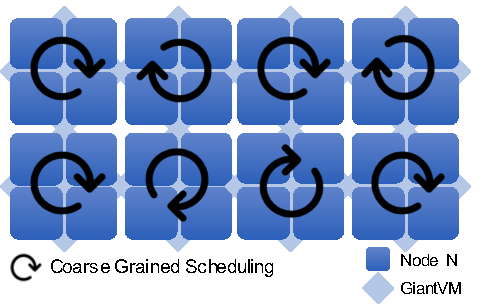
\includegraphics[width=8cm]{coarseschedule.pdf}
  \bicaption[粗粒度调度器的仿真]
    {粗粒度调度器的仿真}
    {Simulation of Coarse-Grained Scheduler}
  \label{fig:simucoarse}
\end{figure}
我们通过设计调度算法来仿真真实环境下巨型虚拟机中shell脚本的功效。如图\ref{fig:simucoarse}所示,集群中每四个节点部署一个巨型虚拟机,这四个节点组成一个$G\_cell$(GiantVM Cell),每次选取负载最低的一个节点作为进程迁移的目的节点。在我们的实现中,$G\_cell$由四个节点组成,每10个时间戳为一个平衡周期,$migrate()$函数在平衡周期的第一个时间戳被调用。其主要算法类似于算法\ref{algo:coarse}但又有所不同:算法\ref{algo:simucoarse}实现了模拟的粗粒度调度器,$migrate()$函数遍历集群中所有的$G\_cell$,在每个$G\_cell$中,找出负载最低的节点,并且$get\_migratable\_tasks()$函数将$G\_cell$中其余三个节点的可迁移进程保存在$removed$集合中。$get\_migratable\_tasks()$函数判断task是否是可迁移进程的标准是其priority小于2且CPU的最大使用率为0.025以下。接下来,统计该节点所有可迁移进程的资源占用量$util\_diff$。将$util\_diff$加到占用最低的节点上,$is\_useful\_migrate()$函数规定出现以下情况时不可迁移:(1)迁移后占用最低节点的占用率比当前节点高;(2)$util\_diff$大于当前节点负载的80\%;(3)迁移后占用最低节点的占用率超过了节点负载量警戒线(目前设置为节点的最大负载能力,$warning\_threshold$)。如果不符合迁移的条件,则该节点上的可迁移进程不被迁移,并在当前$G\_cell$中继续遍历下一个节点。如果符合迁移条件,$removed$集合中的所有进程将被迁移到$G\_cell$内部负载最低的节点上,同时将这次迁移的网络开销加到$bandwidth\_usage$变量上。对于不开启GiantVM平衡功能的集群,$bandwidth\_usage$将为0,远低于开启GiantVM迁移功能的集群,故GiantVM的迁移也可视作牺牲网络带宽来换取CPU使用率的一种方法。

\begin{algorithm}[h]
\begin{algorithmic}[1]
\Function {migrate}{$timestamp$}
\For{each $G\_cell \in Cluster$}
\State $lowest\_loaded\_node \gets find\_lowest\_loaded\_node(G\_cell,\  timestamp)$
\For{each $node \in (G\_cell - lowest\_loaded\_node)$}
\State $/*\ Get\ migratable\ tasks\ */$
\State $util\_diff,\  removed \gets get\_migratable\_tasks(node)$
\State $/*\ No\ migrate\ if\ cannot\ migrate\ or\ profit\ is\ little\ */$
\If{$is\_useful\_migrate(util\_diff,\  removed)$}
\State $bandwidth\_usage \gets bandwidth\_usage + migrate\_to\_node(removed)$
\EndIf
\EndFor
\EndFor
\end{algorithmic}
\caption{粗粒度调度器的仿真算法}
\label{algo:simucoarse}
\end{algorithm}

根据第二章和第三章的分析,粗粒度的调度有助于集群的负载均衡,提高了整体的CPU使用率,且被迁移进程之间不会共享内存。同时,任务的$duration$和机器的$overcommit$都应该下降,因为此调度算法缓解了任务分布不合理所造成的QoS violation,即缓解了单个节点上的CPU需求会短时间爆发性的增长、超过该机器的容载能力的情况,而通过资源重分配利用了长时间处于较低负载状态的机器上多余的资源。仿真算法中,宿主机上的进程可以直接被移送到GiantVM中,被调度到其他节点上,而真实环境下虚拟机和宿主机之间不可以交换进程,这个限制尚未在仿真脚本中进行模拟。事实上,客户机和宿主机之间可以进行网络通信,可以通过网络在客户机与宿主机之间交换进程,这一方案的可行性尚未调查。

\section{细粒度调度器的仿真与调优}
上节所述的粗粒度调度器存在许多可以优化的方面:粗粒度调度器只在$G\_cell$中选取负载最低的节点($lowest\_loaded\_node$),事实上$G\_cell$中可能存在和$lowest\_loaded\_node$负载状况相近的节点,这些负载同样很低的节点没有得到充分利用;其次,粗粒度调度器中对除了$lowest\_loaded\_node$之外的所有节点的任务进行筛选,选出可以迁移的优先级较低的任务迁移到$lowest\_loaded\_node$上。这样会造成较大的网络开销,例如$G\_cell$中有四个节点,则需要将三个节点上的可迁移进程全部进行迁移。这个问题在真实环境下也存在:真实环境下的巨型虚拟机调度器将客户机中所有的进程在NUMA节点之间迁移,而整个操作系统中的进程内存总量是很可观的,从而也会造成单节点上的网络带宽被严重占用。

\subsection{细粒度调度器的仿真}
\begin{figure}[!htp]
  \centering
  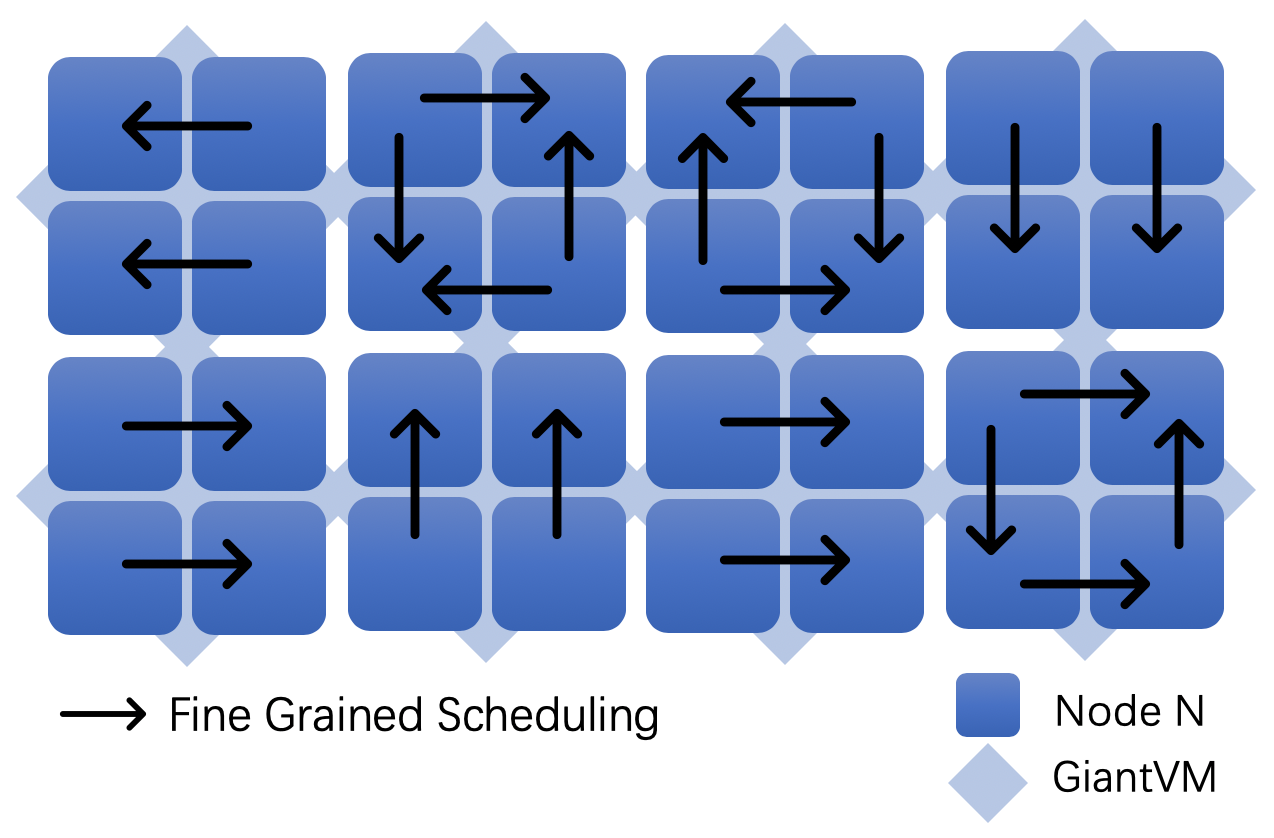
\includegraphics[width=8cm]{fineschedule.png}
  \bicaption[细粒度调度器的仿真]
    {细粒度调度器的仿真}
    {Simulation of Fine-Grained Scheduler}
  \label{fig:simufine}
\end{figure}
为了解决粗粒度调度器所遇到的性能问题,我们设计了细粒度的调度器。算法\ref{algo:simufine}说明了该调度算法的大致过程:和粗粒度的调度算法一样,细粒度算法遍历集群中所有的$G\_cell$,而与粗粒度算法不同的是,我们在一个$G\_cell$中找出负载最低的两个节点,而其他节点分别遍历其所有进程,找出其各自可迁移进程,加入到各自的$removed$集合中,即得到每个节点的可迁移进程的集合$removed$。相对于粗粒度的调度算法,我们认为细粒度的调度算法有较小的网络开销,由于在网络之中迁移的$removed$集合更少。假如一个$G\_cell$中有四个节点,则每个迁移周期中被网络传输的只有两个$removed$集合,而粗粒度的调度算法需要迁移三个$removed$集合。找出节点的$removed$集合后,首先向负载最低的节点迁移$removed$集合中的进程,直到负载最低的节点无法接收新的进程,接下来向负载第二低的节点迁移迁移$removed$集合中的进程,直到第二低负载节点无法接收新的进程。节点是否能接收新进程的判断标准与粗粒度的算法相同,即进程迁移的目的节点的负载不能大于源节点的负载,也不能大于负载警戒线$warning\_threshold$。当负载最低节点和负载第二低节点的接收列表$move\_to\_first$、$move\_to\_second$被填满后,统计两个列表的任务的CPU使用量,当使用量超过一定的阈值才可进行真正的迁移(由$is\_useful\_migrate()$函数判断)。
\begin{algorithm}[h]
\begin{algorithmic}[1]
\Function {migrate}{$timestamp$}
\For{each $G\_cell \in Cluster$}
\State $lowest\_loaded\_node,\ second\_lowest\_loaded\_node \gets find\_lowests(G\_cell,\  timestamp)$
\State
\For{each $node \in (G\_cell - lowest\_loaded\_node - second\_lowest\_loaded\_node)$}
\State $/*\ Get\ migratable\ tasks\ while\ target\ nodes\ can\ hold\ */$
\State $removed \gets get\_migratable\_tasks(node)$
\While{$first\_lowest\_can\_hold()\ and\ !removed.empty()$}
\State $move\_to\_first.add(removed.pop())$
\EndWhile
\While{$second\_lowest\_can\_hold()\ and\ !removed.empty()$}
\State $move\_to\_second.add(removed.pop())$
\EndWhile
\State
\State $/*\ No\ migrate\ if\ profit\ is\ little\ */$
\If{$is\_useful\_migrate(util(move\_to\_first))$}
\State $bandwidth\_usage \gets bandwidth\_usage + migrate\_to\_first(move\_to\_first)$
\EndIf
\If{$is\_useful\_migrate(util(move\_to\_second)$}
\State $bandwidth\_usage \gets bandwidth\_usage + migrate\_to\_second(move\_to\_second)$
\EndIf
\EndFor
\EndFor
\end{algorithmic}
\caption{细粒度调度器的仿真算法}
\label{algo:simufine}
\end{algorithm}

如图\ref{fig:simufine}所示,细粒度的调度算法发生在两组节点之间。举例而言,对于$G\_cell$大小为4的集群,节点编号为node0-3,假设负载情况是node0\,<\,node1\,<\,node2\,<\,node3,那么进程将会由node2,3向node0,1迁移。而对比粗粒度的调度算法,只有node0作为接收进程的节点,需要同时接收来自于node1-3的可迁移进程。假设所有的节点不存在无法接收被迁移进程的情况(即资源充足),那么node0将会接收3个$removed$集合的进程,不但对node0的网络带宽造成较大压力,也使得node0的CPU负载迅速升高,但其他节点的CPU使用率一律降低,造成了CPU使用率的不均衡。而对于细粒度调度算法,node0,1平均只需接收来自于一个节点的$removed$集合,网络开销明显减小,且node0,1分担了CPU负载,CPU负载不会大幅度上升。所以我们认为,细粒度的调度算法具有更强的集群负载平衡能力,也具有较小的网络开销。

\subsection{排序的细粒度调度算法}
在众多的调度器中,排序是提高调度器效率的重要方法,例如Linux\cite{linux}的完全公平调度器使用红黑树将进程按照$vruntime$排序,使得进程公平地拥有运行时间。在巨型虚拟机的调度算法中,依然可以应用排序。根据谷歌提供的集群追踪数据,我们有两种排序的方案:

\noindent\textbf{根据CPU数据排序}\quad 谷歌的集群追踪数据中可用于CPU使用情况排序的数据有:$task\_usage$表中的进程每个时刻的CPU使用率$Task.usage[cpu]$,以及$task\_events$表中进程CPU使用率上限$Task.request$。我们认为,将CPU使用率较低的进程优先调度有助于提高集群的CPU使用率。举例而言,假设最低的节点剩余的CPU负载能力为1,而可供迁移的进程的CPU使用量是0.6,0.45,0.43。如果CPU使用率高的进程优先调度,则被迁移到负载最低节点上的进程为0.6,还剩余0.4未占用的CPU负载能力;如果CPU使用率低的进程优先调度,则进程0.45,0.43被调度,占用了0.87的空闲CPU,高于按照CPU使用率高的优先调度的情况。这是因为CPU使用率高的进程会在空余的CPU负载能力中造成较大的碎片,例如在这个例子中,0.6的进程造成了0.4的碎片,是空闲CPU使用量的40\%。假如可迁移进程的CPU使用量分别是1.1,0.9,0.1,那么如果CPU使用率高的进程优先调度,则不会有进程被调度;而CPU使用率低的进程优先调度则可以占满所有空闲的CPU。事实上,向空余CPU中填充进程的问题是一个背包问题,即:背包可以容纳重量为1的物品,每件物品的价值和重量相等,分别为0.6,0.45,0.43。背包问题一个NP完全问题,本文优先调度CPU占用较低的进程,用贪心法求得近似解。对于表征CPU使用量的数据的选取,我们认为$Task.usage[cpu]$比$Task.request$更具有代表性,因为$Task.usage$是实时获取的数据,更有利于动态计算集群中的任务负载情况。

\noindent\textbf{根据内存数据排序}\quad 对内存使用情况进行排序的主要目的是降低网络的开销。我们使用的谷歌的集群追踪数据主要提供了进程的两个内存使用情况的数据:$Task.usage[memory]$每个时刻下进程容器所使用的总的内存页数量,称作assigned memory,包含该任务的用户态和内核态页面,也是谷歌Borg集群中容器迁移所要迁移的真正的页面数量(见\ref{chap:containermigration}节的背景介绍);$Task.usage[MPI]$,平均每条指令的访存次数(memory accesses per instruction),通过performance counter获得\footnote{performance counter\cite{perf}是CPU硬件上的一组寄存器,记录了各类硬件事件,包括分支预测错误、缓存不命中次数、指令执行次数等。}。一个进程所拥有的内存页的数量与缓存不命中的频率有一些关联度(正相关),但关联度不是很高:CPU密集型任务拥有的内存页较少,MPI也较低;内存密集型任务的MPI较高,但其经常访问的内存页的数目不一定大,也存在拥有大量内存页的进程的MPI较低的情况,故MPI反映了进程频繁访问内存页面的数量。如果优先调度内存占用$Task.usage[memory]$或$Task.usage[MPI]$高的进程,将会有效地减小迁移的网络开销。由于细粒度的调度器将可调度进程分为两组(在真实情况下,巨型虚拟机的任务将在两个NUMA节点上运行),这两组进程可能会产生大量的共享内存访问(见\ref{chap:memm}节)。但是由于谷歌的追踪数据未提供进程访问内存的具体位置,所以我们无法对此情况进行仿真。

排序的细粒度调度算法由算法\ref{algo:sorted}表述。在每个迁移循环中,将$removed$队列按照$sort\_option$排序,将$removed$队列首部的第一个进程$pop()$出来,依次添加到$move\_to\_first$集合和$move\_to\_second$集合中等待迁移,除此之外和未排序的细粒度仿真算法相同。我们提供了6个$sort\_option$,作为测试比较的对象,分别为:

\begin{itemize}
  \item 0:不排序;
  \item 1:按照进程的CPU使用率上限(CPU request)从小到大排序;
  \item 2:按照$timestamp$时刻的CPU使用量从小到大排序
  \item 3:按照$timestamp$时刻的内存使用量从小到大排序
  \item 4:按照$timestamp$时刻的CPU使用量从大到小排序
  \item 5:按照$timestamp$时刻的MPI从小到大排序
\end{itemize}

\begin{algorithm}[h]
\begin{algorithmic}[1]
\Function {migrate}{$timestamp$}
\State $...... /* Same \ as\  algorithm\ $\ref{algo:simufine}$\ */$
\State $removed \gets get\_sorted\_migratable\_tasks(node,\ sort\_option)$
\While{$first\_lowest\_can\_hold()\ and\ !removed.empty()$}
\State $move\_to\_first.add(removed.pop(0))$
\EndWhile
\While{$second\_lowest\_can\_hold()\ and\ !removed.empty()$}
\State $move\_to\_second.add(removed.pop(0))$
\EndWhile
\State $...... /* Same \ as\  algorithm\ $\ref{algo:simufine}$\ */$
\end{algorithmic}
\caption{排序的细粒度调度器}
\label{algo:sorted}
\end{algorithm}

\section{本章小结}
本章通过仿真一个具有800个相同机器的集群,通过Python脚本实现了便利、快捷且有效的仿真条件,模拟了第三章真实环境下的巨型虚拟机平衡调度器。分析了粗粒度调度器存在的性能问题,如网络开销太大、集群资源利用率仍不平衡,并设计了细粒度的进程调度器。分析了进程调度顺序对平衡效果以及网络开销的影响,设计了排序的细粒度调度器,并且提供了6种不同的排序选项。我们将在下一章对这6个排序选项进行性能测试和分析。
\include{body/conclusion} %% 全文总结


%%%%%%%%%%%%%%%%%%%%%%%%%%%%%% 
%% 附录(章节编号重新计算,使用字母进行编号)
%%%%%%%%%%%%%%%%%%%%%%%%%%%%%% 
\appendix

% 附录中编号形式是"A-1"的样子
\renewcommand\theequation{\Alph{chapter}--\arabic{equation}}
\renewcommand\thefigure{\Alph{chapter}--\arabic{figure}}
\renewcommand\thetable{\Alph{chapter}--\arabic{table}}

\include{body/app1} % 更新记录
\include{body/app2} % 麦克斯韦方程
% \include{body/app3}


%%%%%%%%%%%%%%%%%%%%%%%%%%%%%% 
%% 文后(无章节编号)
%%%%%%%%%%%%%%%%%%%%%%%%%%%%%% 
\backmatter

% 参考文献
% 使用 BibTeX
% 包含参考文献文件.bib
\bibliography{reference/chap1,reference/chap2}

%% 个人简历(学士学位论文没有个人简历要求)
% \include{body/resume}

% 致谢
%# -*- coding: utf-8-unix -*-
\begin{thanks}
在我大学四年的学习生活里以及毕业设计的完成过程中,我遇到了许许多多优秀的老师和同学,以及很多给予了我帮助的人,在此对他们表示感谢。

感谢戚正伟教授对我毕业设计的指导以及学业中的诸多事宜的关心,是您的悉心关注和严格要求让我按时高质量地完成了毕业设计,在科研工作中您同我们一起进行实验,一起解决问题,提升了我的技术写作能力、表达能力,让我有了更好的代码规范,对我的学业有莫大的帮助,鼓励我不断解决问题,作出新的成绩。

感谢上海市重点可扩展计算与系统实验室的学长们,你们对我有求必应,帮我解决了诸多我没有能力解决的问题。感谢张晋学长,没有他的建议和提示,就没有本文的结果。也要感谢其他项目组的学长,虽然他们没有对我的研究项目进行具体的帮助,但他们的热心与鼓励依然提高了我攻坚克难的信心。也要感谢陈育彬学长和丁卓成学长,你们的毕业论文和技术文档、代码对我了解巨型虚拟机有极大的帮助,是我的指明灯。

感谢和我同级的余博识同学,他和我共同协作,讨论了许许多多的问题,为我提供了新的研究思路。在实验室期间,他和我合作完成了实验环境的配置,实验数据的统计,以及项目文档的撰写。他和我朝夕相处,是我最好的战友和伙伴。

感谢在交大期间遇到的同学和朋友,是你们让我的生活更加丰富,是你们和我一起完成各项大作业,和我一起自习一起健身,一起吃饭一起娱乐,让我收获了美好真挚的友谊。

感谢宿舍的宿管阿姨,以及食堂的阿姨,是你们照顾同学们的饮食起居,保证了学校生活的安全和便利,对我们无微不至地照顾。感谢你们!

还有其他许许多多的老师与同学,你们是我大学生活的记忆,祝愿你们前途似锦,生活愉快,事业有成!

上海市重点可扩展计算与系统实验室
  

\end{thanks}


% 发表文章目录
%%# -*- coding: utf-8-unix -*-
%%==================================================
%% pub.tex for SJTUThesis
%% Encoding: UTF-8
%%==================================================

\begin{publications}{99}
    \item\textsc{Chen H, Chan C~T}. {Acoustic cloaking in three dimensions using acoustic metamaterials}[J]. Applied Physics Letters, 2007, 91:183518.
    \item\textsc{Chen H, Wu B~I, Zhang B}, et al. {Electromagnetic Wave Interactions with a Metamaterial Cloak}[J]. Physical Review Letters, 2007, 99(6):63903.
\end{publications}


% 参与项目列表
%%# -*- coding: utf-8-unix -*-
%%==================================================
%% projects.tex for SJTUThesis
%% Encoding: UTF-8
%%==================================================

\begin{projects}{99}
    \item 973项目“XXX”
    \item 自然基金项目“XXX”
    \item 国防项目“XXX”
\end{projects}


%英文大摘要
\include{body/bigabstract}

\end{document}
